% Options for packages loaded elsewhere
\PassOptionsToPackage{unicode}{hyperref}
\PassOptionsToPackage{hyphens}{url}
%
\documentclass[
]{book}
\usepackage{lmodern}
\usepackage{amssymb,amsmath}
\usepackage{ifxetex,ifluatex}
\ifnum 0\ifxetex 1\fi\ifluatex 1\fi=0 % if pdftex
  \usepackage[T1]{fontenc}
  \usepackage[utf8]{inputenc}
  \usepackage{textcomp} % provide euro and other symbols
\else % if luatex or xetex
  \usepackage{unicode-math}
  \defaultfontfeatures{Scale=MatchLowercase}
  \defaultfontfeatures[\rmfamily]{Ligatures=TeX,Scale=1}
\fi
% Use upquote if available, for straight quotes in verbatim environments
\IfFileExists{upquote.sty}{\usepackage{upquote}}{}
\IfFileExists{microtype.sty}{% use microtype if available
  \usepackage[]{microtype}
  \UseMicrotypeSet[protrusion]{basicmath} % disable protrusion for tt fonts
}{}
\makeatletter
\@ifundefined{KOMAClassName}{% if non-KOMA class
  \IfFileExists{parskip.sty}{%
    \usepackage{parskip}
  }{% else
    \setlength{\parindent}{0pt}
    \setlength{\parskip}{6pt plus 2pt minus 1pt}}
}{% if KOMA class
  \KOMAoptions{parskip=half}}
\makeatother
\usepackage{xcolor}
\IfFileExists{xurl.sty}{\usepackage{xurl}}{} % add URL line breaks if available
\IfFileExists{bookmark.sty}{\usepackage{bookmark}}{\usepackage{hyperref}}
\hypersetup{
  pdftitle={Introdução ao R com aplicações em biodiversidade e conservação},
  hidelinks,
  pdfcreator={LaTeX via pandoc}}
\urlstyle{same} % disable monospaced font for URLs
\usepackage{color}
\usepackage{fancyvrb}
\newcommand{\VerbBar}{|}
\newcommand{\VERB}{\Verb[commandchars=\\\{\}]}
\DefineVerbatimEnvironment{Highlighting}{Verbatim}{commandchars=\\\{\}}
% Add ',fontsize=\small' for more characters per line
\usepackage{framed}
\definecolor{shadecolor}{RGB}{248,248,248}
\newenvironment{Shaded}{\begin{snugshade}}{\end{snugshade}}
\newcommand{\AlertTok}[1]{\textcolor[rgb]{0.94,0.16,0.16}{#1}}
\newcommand{\AnnotationTok}[1]{\textcolor[rgb]{0.56,0.35,0.01}{\textbf{\textit{#1}}}}
\newcommand{\AttributeTok}[1]{\textcolor[rgb]{0.77,0.63,0.00}{#1}}
\newcommand{\BaseNTok}[1]{\textcolor[rgb]{0.00,0.00,0.81}{#1}}
\newcommand{\BuiltInTok}[1]{#1}
\newcommand{\CharTok}[1]{\textcolor[rgb]{0.31,0.60,0.02}{#1}}
\newcommand{\CommentTok}[1]{\textcolor[rgb]{0.56,0.35,0.01}{\textit{#1}}}
\newcommand{\CommentVarTok}[1]{\textcolor[rgb]{0.56,0.35,0.01}{\textbf{\textit{#1}}}}
\newcommand{\ConstantTok}[1]{\textcolor[rgb]{0.00,0.00,0.00}{#1}}
\newcommand{\ControlFlowTok}[1]{\textcolor[rgb]{0.13,0.29,0.53}{\textbf{#1}}}
\newcommand{\DataTypeTok}[1]{\textcolor[rgb]{0.13,0.29,0.53}{#1}}
\newcommand{\DecValTok}[1]{\textcolor[rgb]{0.00,0.00,0.81}{#1}}
\newcommand{\DocumentationTok}[1]{\textcolor[rgb]{0.56,0.35,0.01}{\textbf{\textit{#1}}}}
\newcommand{\ErrorTok}[1]{\textcolor[rgb]{0.64,0.00,0.00}{\textbf{#1}}}
\newcommand{\ExtensionTok}[1]{#1}
\newcommand{\FloatTok}[1]{\textcolor[rgb]{0.00,0.00,0.81}{#1}}
\newcommand{\FunctionTok}[1]{\textcolor[rgb]{0.00,0.00,0.00}{#1}}
\newcommand{\ImportTok}[1]{#1}
\newcommand{\InformationTok}[1]{\textcolor[rgb]{0.56,0.35,0.01}{\textbf{\textit{#1}}}}
\newcommand{\KeywordTok}[1]{\textcolor[rgb]{0.13,0.29,0.53}{\textbf{#1}}}
\newcommand{\NormalTok}[1]{#1}
\newcommand{\OperatorTok}[1]{\textcolor[rgb]{0.81,0.36,0.00}{\textbf{#1}}}
\newcommand{\OtherTok}[1]{\textcolor[rgb]{0.56,0.35,0.01}{#1}}
\newcommand{\PreprocessorTok}[1]{\textcolor[rgb]{0.56,0.35,0.01}{\textit{#1}}}
\newcommand{\RegionMarkerTok}[1]{#1}
\newcommand{\SpecialCharTok}[1]{\textcolor[rgb]{0.00,0.00,0.00}{#1}}
\newcommand{\SpecialStringTok}[1]{\textcolor[rgb]{0.31,0.60,0.02}{#1}}
\newcommand{\StringTok}[1]{\textcolor[rgb]{0.31,0.60,0.02}{#1}}
\newcommand{\VariableTok}[1]{\textcolor[rgb]{0.00,0.00,0.00}{#1}}
\newcommand{\VerbatimStringTok}[1]{\textcolor[rgb]{0.31,0.60,0.02}{#1}}
\newcommand{\WarningTok}[1]{\textcolor[rgb]{0.56,0.35,0.01}{\textbf{\textit{#1}}}}
\usepackage{longtable,booktabs}
% Correct order of tables after \paragraph or \subparagraph
\usepackage{etoolbox}
\makeatletter
\patchcmd\longtable{\par}{\if@noskipsec\mbox{}\fi\par}{}{}
\makeatother
% Allow footnotes in longtable head/foot
\IfFileExists{footnotehyper.sty}{\usepackage{footnotehyper}}{\usepackage{footnote}}
\makesavenoteenv{longtable}
\usepackage{graphicx,grffile}
\makeatletter
\def\maxwidth{\ifdim\Gin@nat@width>\linewidth\linewidth\else\Gin@nat@width\fi}
\def\maxheight{\ifdim\Gin@nat@height>\textheight\textheight\else\Gin@nat@height\fi}
\makeatother
% Scale images if necessary, so that they will not overflow the page
% margins by default, and it is still possible to overwrite the defaults
% using explicit options in \includegraphics[width, height, ...]{}
\setkeys{Gin}{width=\maxwidth,height=\maxheight,keepaspectratio}
% Set default figure placement to htbp
\makeatletter
\def\fps@figure{htbp}
\makeatother
\setlength{\emergencystretch}{3em} % prevent overfull lines
\providecommand{\tightlist}{%
  \setlength{\itemsep}{0pt}\setlength{\parskip}{0pt}}
\setcounter{secnumdepth}{5}
\usepackage{booktabs}
\usepackage{amsthm}
\makeatletter
\def\thm@space@setup{%
  \thm@preskip=8pt plus 2pt minus 4pt
  \thm@postskip=\thm@preskip
}
\makeatother
\usepackage[]{natbib}
\bibliographystyle{apalike}

\title{Introdução ao R com aplicações em biodiversidade e conservação}
\author{}
\date{\vspace{-2.5em}2020-06-18}

\begin{document}
\maketitle

{
\setcounter{tocdepth}{1}
\tableofcontents
}
\hypertarget{pruxe9-requisitos}{%
\chapter{Pré-requisitos}\label{pruxe9-requisitos}}

This is a \emph{sample} book written in \textbf{Markdown}. You can use anything that Pandoc's Markdown supports, e.g., a math equation \(a^2 + b^2 = c^2\).

The \textbf{bookdown} package can be installed from CRAN or Github:

\begin{Shaded}
\begin{Highlighting}[]
\KeywordTok{install.packages}\NormalTok{(}\StringTok{"bookdown"}\NormalTok{)}
\CommentTok{# or the development version}
\CommentTok{# devtools::install_github("rstudio/bookdown")}
\end{Highlighting}
\end{Shaded}

Remember each Rmd file contains one and only one chapter, and a chapter is defined by the first-level heading \texttt{\#}.

To compile this example to PDF, you need XeLaTeX. You are recommended to install TinyTeX (which includes XeLaTeX): \url{https://yihui.name/tinytex/}.

\hypertarget{perguntas}{%
\chapter{Perguntas}\label{perguntas}}

\hypertarget{introduuxe7uxe3o-ao-tidyverse}{%
\chapter{Introdução ao Tidyverse}\label{introduuxe7uxe3o-ao-tidyverse}}

\hypertarget{backgorund-da-anuxe1lise}{%
\section{Backgorund da análise}\label{backgorund-da-anuxe1lise}}

Lorem ipsum dolor sit amet, consectetur adipiscing elit. Proin in nisi egestas, volutpat lectus non, interdum nunc. Lorem ipsum dolor sit amet, consectetur adipiscing elit. Ut nulla quam, fermentum consequat maximus tristique, ultricies eget nunc. Donec efficitur tristique est hendrerit eleifend. Mauris elementum arcu vitae ultrices congue. Proin accumsan sollicitudin augue et iaculis. Quisque id tempor elit. Interdum et malesuada fames ac ante ipsum primis in faucibus. Duis iaculis purus nisi, non luctus metus vulputate quis. Maecenas felis urna, tristique eu maximus non, placerat aliquet felis. Ut elit enim, consequat in metus facilisis, fringilla dignissim neque. Nunc vehicula nulla et euismod interdum. Donec quis sapien non mi aliquet laoreet. Sed fermentum diam eu tempor hendrerit. Sed varius orci sit amet massa pellentesque, commodo commodo velit auctor. Integer finibus erat vitae sapien mattis, et auctor augue tincidun.

\hypertarget{exemplo-1}{%
\section{Exemplo 1:}\label{exemplo-1}}

\begin{itemize}
\tightlist
\item
  Pergunta:
\item
  Predição:
\item
  Variáveis preditoras:
\item
  Variáveis dependens:
\end{itemize}

\hypertarget{explicauxe7uxe3o-da-anuxe1lise}{%
\subsection{Explicação da análise}\label{explicauxe7uxe3o-da-anuxe1lise}}

Lorem ipsum dolor sit amet, consectetur adipiscing elit. Proin in nisi egestas, volutpat lectus non, interdum nunc. Lorem ipsum dolor sit amet, consectetur adipiscing elit.

\textbf{Checklist}

\begin{itemize}
\tightlist
\item
  Verificar distribuição dos dados\\
\item
  item 2\\
\item
  item 3
\end{itemize}

\hypertarget{anuxe1lise}{%
\subsection{Análise}\label{anuxe1lise}}

\hypertarget{interpretauxe7uxe3o-dos-resultados}{%
\subsubsection{Interpretação dos resultados}\label{interpretauxe7uxe3o-dos-resultados}}

Lorem ipsum dolor sit amet, consectetur adipiscing elit. Proin in nisi egestas, volutpat lectus non, interdum nunc. Lorem ipsum dolor sit amet, consectetur adipiscing elit.

\hypertarget{para-se-aprofundar}{%
\subsection{Para se aprofundar}\label{para-se-aprofundar}}

\begin{itemize}
\item
\end{itemize}

\hypertarget{anuxe1lises-univariadas-lm}{%
\chapter{Análises Univariadas (LM)}\label{anuxe1lises-univariadas-lm}}

Lorem ipsum dolor sit amet, consectetur adipiscing elit. Proin in nisi egestas, volutpat lectus non, interdum nunc. Lorem ipsum dolor sit amet, consectetur adipiscing elit. Ut nulla quam, fermentum consequat maximus tristique, ultricies eget nunc. Donec efficitur tristique est hendrerit eleifend. Mauris elementum arcu vitae ultrices congue. Proin accumsan sollicitudin augue et iaculis. Quisque id tempor elit. Interdum et malesuada fames ac ante ipsum primis in faucibus. Duis iaculis purus nisi, non luctus metus vulputate quis. Maecenas felis urna, tristique eu maximus non, placerat aliquet felis. Ut elit enim, consequat in metus facilisis, fringilla dignissim neque. Nunc vehicula nulla et euismod interdum. Donec quis sapien non mi aliquet laoreet. Sed fermentum diam eu tempor hendrerit. Sed varius orci sit amet massa pellentesque, commodo commodo velit auctor. Integer finibus erat vitae sapien mattis, et auctor augue tincidunt.

\hypertarget{sub-seuxe7uxe3o-1}{%
\section{Sub-seção 1}\label{sub-seuxe7uxe3o-1}}

Duis scelerisque porta massa id lacinia. Quisque sodales malesuada neque, at posuere justo. Sed nec diam vel sapien feugiat efficitur lobortis a massa. Vestibulum in finibus urna, in facilisis quam. Sed purus libero, lacinia id arcu in, volutpat tempor elit. Donec luctus tellus quis arcu porttitor aliquet. Duis pellentesque felis non dolor ullamcorper pharetra. Proin sit amet justo id metus tempus faucibus eget a dolor. Cras elementum massa et justo tempor placerat. Etiam ac metus interdum, efficitur magna sed, mattis velit.

\hypertarget{sub-seuxe7uxe3o-2}{%
\section{Sub-seção 2}\label{sub-seuxe7uxe3o-2}}

Duis nec nisi sapien. Aenean a metus faucibus, malesuada ante et, semper magna. Sed vel fermentum mauris. Duis consectetur eget risus condimentum tempus. Cras tincidunt dui sed rutrum mollis. Sed tincidunt condimentum odio at luctus. Quisque sed augue urna. Aenean vel turpis dignissim, finibus elit commodo, sagittis massa. Sed lacinia leo massa, a varius sapien dictum in. Sed at pellentesque velit. Quisque pretium est a nisi fringilla, at bibendum enim sagittis. Phasellus a facilisis orci. Mauris auctor dolor a nunc cursus, in mattis lorem euismod. Donec sed convallis felis.

\hypertarget{sub-seuxe7uxe3o-3}{%
\section{Sub-seção 3}\label{sub-seuxe7uxe3o-3}}

Nam tortor lacus, volutpat ac aliquam tincidunt, posuere eu dui. Donec auctor ante convallis diam laoreet, eget luctus lorem iaculis. Proin feugiat ipsum nec velit commodo bibendum. Phasellus aliquet metus vehicula convallis aliquam. Quisque pretium ut augue non mollis. Nulla ut pulvinar nisl, at blandit sem. Nam vitae pellentesque risus. Fusce rhoncus eros eget velit volutpat rhoncus. Nam tempor varius fringilla. Aliquam venenatis interdum lorem at pellentesque. Nam a risus vitae dolor maximus ullamcorper nec et diam. Nunc condimentum arcu eu lacinia pellentesque. Etiam at nulla felis.

\hypertarget{anuxe1lises-univariadas-modelos-mistos-generalizados}{%
\chapter{Análises Univariadas (modelos mistos generalizados)}\label{anuxe1lises-univariadas-modelos-mistos-generalizados}}

Lorem ipsum dolor sit amet, consectetur adipiscing elit. Proin in nisi egestas, volutpat lectus non, interdum nunc. Lorem ipsum dolor sit amet, consectetur adipiscing elit. Ut nulla quam, fermentum consequat maximus tristique, ultricies eget nunc. Donec efficitur tristique est hendrerit eleifend. Mauris elementum arcu vitae ultrices congue. Proin accumsan sollicitudin augue et iaculis. Quisque id tempor elit. Interdum et malesuada fames ac ante ipsum primis in faucibus. Duis iaculis purus nisi, non luctus metus vulputate quis. Maecenas felis urna, tristique eu maximus non, placerat aliquet felis. Ut elit enim, consequat in metus facilisis, fringilla dignissim neque. Nunc vehicula nulla et euismod interdum. Donec quis sapien non mi aliquet laoreet. Sed fermentum diam eu tempor hendrerit. Sed varius orci sit amet massa pellentesque, commodo commodo velit auctor. Integer finibus erat vitae sapien mattis, et auctor augue tincidunt.

\hypertarget{sub-seuxe7uxe3o-1-1}{%
\section{Sub-seção 1}\label{sub-seuxe7uxe3o-1-1}}

Duis scelerisque porta massa id lacinia. Quisque sodales malesuada neque, at posuere justo. Sed nec diam vel sapien feugiat efficitur lobortis a massa. Vestibulum in finibus urna, in facilisis quam. Sed purus libero, lacinia id arcu in, volutpat tempor elit. Donec luctus tellus quis arcu porttitor aliquet. Duis pellentesque felis non dolor ullamcorper pharetra. Proin sit amet justo id metus tempus faucibus eget a dolor. Cras elementum massa et justo tempor placerat. Etiam ac metus interdum, efficitur magna sed, mattis velit.

\hypertarget{sub-seuxe7uxe3o-2-1}{%
\section{Sub-seção 2}\label{sub-seuxe7uxe3o-2-1}}

Duis nec nisi sapien. Aenean a metus faucibus, malesuada ante et, semper magna. Sed vel fermentum mauris. Duis consectetur eget risus condimentum tempus. Cras tincidunt dui sed rutrum mollis. Sed tincidunt condimentum odio at luctus. Quisque sed augue urna. Aenean vel turpis dignissim, finibus elit commodo, sagittis massa. Sed lacinia leo massa, a varius sapien dictum in. Sed at pellentesque velit. Quisque pretium est a nisi fringilla, at bibendum enim sagittis. Phasellus a facilisis orci. Mauris auctor dolor a nunc cursus, in mattis lorem euismod. Donec sed convallis felis.

\hypertarget{sub-seuxe7uxe3o-3-1}{%
\section{Sub-seção 3}\label{sub-seuxe7uxe3o-3-1}}

Nam tortor lacus, volutpat ac aliquam tincidunt, posuere eu dui. Donec auctor ante convallis diam laoreet, eget luctus lorem iaculis. Proin feugiat ipsum nec velit commodo bibendum. Phasellus aliquet metus vehicula convallis aliquam. Quisque pretium ut augue non mollis. Nulla ut pulvinar nisl, at blandit sem. Nam vitae pellentesque risus. Fusce rhoncus eros eget velit volutpat rhoncus. Nam tempor varius fringilla. Aliquam venenatis interdum lorem at pellentesque. Nam a risus vitae dolor maximus ullamcorper nec et diam. Nunc condimentum arcu eu lacinia pellentesque. Etiam at nulla felis.

\hypertarget{anuxe1lises-multivariadas}{%
\chapter{Análises Multivariadas}\label{anuxe1lises-multivariadas}}

We have finished a nice book.

\hypertarget{rarefauxe7uxe3o}{%
\chapter{Rarefação}\label{rarefauxe7uxe3o}}

\hypertarget{backgorund-da-anuxe1lise-1}{%
\section{Backgorund da análise}\label{backgorund-da-anuxe1lise-1}}

Um das dificuldades na comparação da riqueza de espécies entre comunidades é decorrente da diferença no esforço amostral (e.g.diferença no número de indivíduos, discrepância na quantidade de unidades amostrais ou área amostrada) que inevitavelmente influenciará no número de espécies observadas (Gotelli \& Chao 2013). O método de rarefação nos permite comparar o número de espécies entre comunidades quando o tamanho da amostra ou a abundância de indivíduos não são iguais. A rarefação calcula o número esperado de espécies em cada comunidade tendo como base comparativa um valor em que todas as amostras atinjam um tamanho padrão, ou comparações baseadas na menor amostra ou com menos indivíduos (dentre todas amostras possíveis). O teste foi formulado considerando seguinte pergunta: Se considerarmos \emph{n} indivíduos ou amostras (\emph{n} \textless{} N) para cada comunidade, quantas espécies registraríamos nas comunidades considerando o mesmo número de indivíduos ou amostras?

\begin{quote}
\[E(S) = \sum 1 - \frac{{(N - N_1)}/{n}}{{N}/{n}}\]
\end{quote}

Onde:

\begin{itemize}
\item
  E(S) = Número de espécies esperado,
\item
  N = Número total de indivíduos na amostra,
\item
  Ni = Número de indivíduos da iésima espécie,
\item
  \emph{n} = tamanho da amostra padronizada (menor amostra).
\end{itemize}

Gotelli \& Collwel (2001) descrevem este método e discutem em detalhes as restrições sobre seu uso na ecologia: i) as amostras a serem comparados devem ser consistentes do ponto de vista taxonômico, ou seja, todos os indivíduos devem pertencer ao mesmo grupo taxonômico; ii) as comparações devem ser realizadas somente entre amostras com as mesmas técnicas de coleta; iii) os tipos de hábitat onde as amostras são obtidas devem ser semelhantes; e iv) é um método para estimar a riqueza de espécies em uma amostra menor -- não pode ser usado para extrapolar e estimar riqueza. Contudo, é importante ressaltar que esta última restrição foi superada por Colwell et al.~(2012) e Chao \& Jost (2012) que desenvolveram uma nova abordagem onde os dados podem ser interpolados (rarefeito) para amostras menores e extrapolados para amostras maiores.

~

\hypertarget{exemplo-pruxe1tico---rarefauxe7uxe3o}{%
\subsubsection{Exemplo prático - Rarefação}\label{exemplo-pruxe1tico---rarefauxe7uxe3o}}

\hypertarget{explicauxe7uxe3o-dos-dados}{%
\paragraph{Explicação dos dados}\label{explicauxe7uxe3o-dos-dados}}

Neste exemplo usaremos os dados de espécies de morcegos amostradas em três fragmentos florestais (Breviglieri 2008): i) Mata Ciliar do Córrego Talhadinho com 12 hectares inserida em uma matriz de pastagem; ii) Mata Ciliar do Córrego dos Tenentes com 10 hectares inserida em uma matriz de cultivo de cana-de-açucar e pastagem; e iii) Fazenda Experimental de Pindorama com 128 hectares inserida uma matriz de cana-de-açúcar e pastagem.

\textbf{Pergunta:}

\begin{quote}
A riqueza de espécies de morcegos é maior na Fazenda Experimental do que nos fragmentos florestais menores?
\end{quote}

\textbf{Predições}

\begin{quote}
O número de espécies será maior em fragmentos florestais maiores.
\end{quote}

\textbf{Variáveis}

\begin{itemize}
\tightlist
\item
  Variáveis preditoras

  \begin{itemize}
  \tightlist
  \item
    matriz ou dataframe com as abundâncias das espécies de morcegos registradas nos três fragmentos florestais
  \end{itemize}
\end{itemize}

\textbf{Checklist}

\begin{itemize}
\tightlist
\item
  Verificar se a sua matriz ou dataframe estão com as espécies nas linhas e os fragmentos florestais nas colunas
\end{itemize}

\hypertarget{anuxe1lise-1}{%
\subsection{Análise}\label{anuxe1lise-1}}

Calculo da rarefação

\begin{Shaded}
\begin{Highlighting}[]
\KeywordTok{library}\NormalTok{(ecodados)}
\KeywordTok{library}\NormalTok{(iNEXT)}
\NormalTok{dados_rarefacao <-}\StringTok{ }\NormalTok{rarefacao_morcegos}
\NormalTok{resultados_rarefacao <-}\StringTok{ }\KeywordTok{iNEXT}\NormalTok{(dados_rarefacao, }\DataTypeTok{q =} \DecValTok{0}\NormalTok{, }\DataTypeTok{datatype =} \StringTok{"abundance"}\NormalTok{, }\DataTypeTok{endpoint =} \DecValTok{800}\NormalTok{)}

\CommentTok{# Visualizar os resultados }
\KeywordTok{ggiNEXT}\NormalTok{(resultados_rarefacao, }\DataTypeTok{type =} \DecValTok{1}\NormalTok{, }\DataTypeTok{facet.var =} \StringTok{"order"}\NormalTok{)}
\end{Highlighting}
\end{Shaded}

\begin{verbatim}
## Warning in ggiNEXT.iNEXT(resultados_rarefacao, type = 1, facet.var = "order"):
## invalid facet.var setting, the iNEXT object do not consist multiple orders.
\end{verbatim}

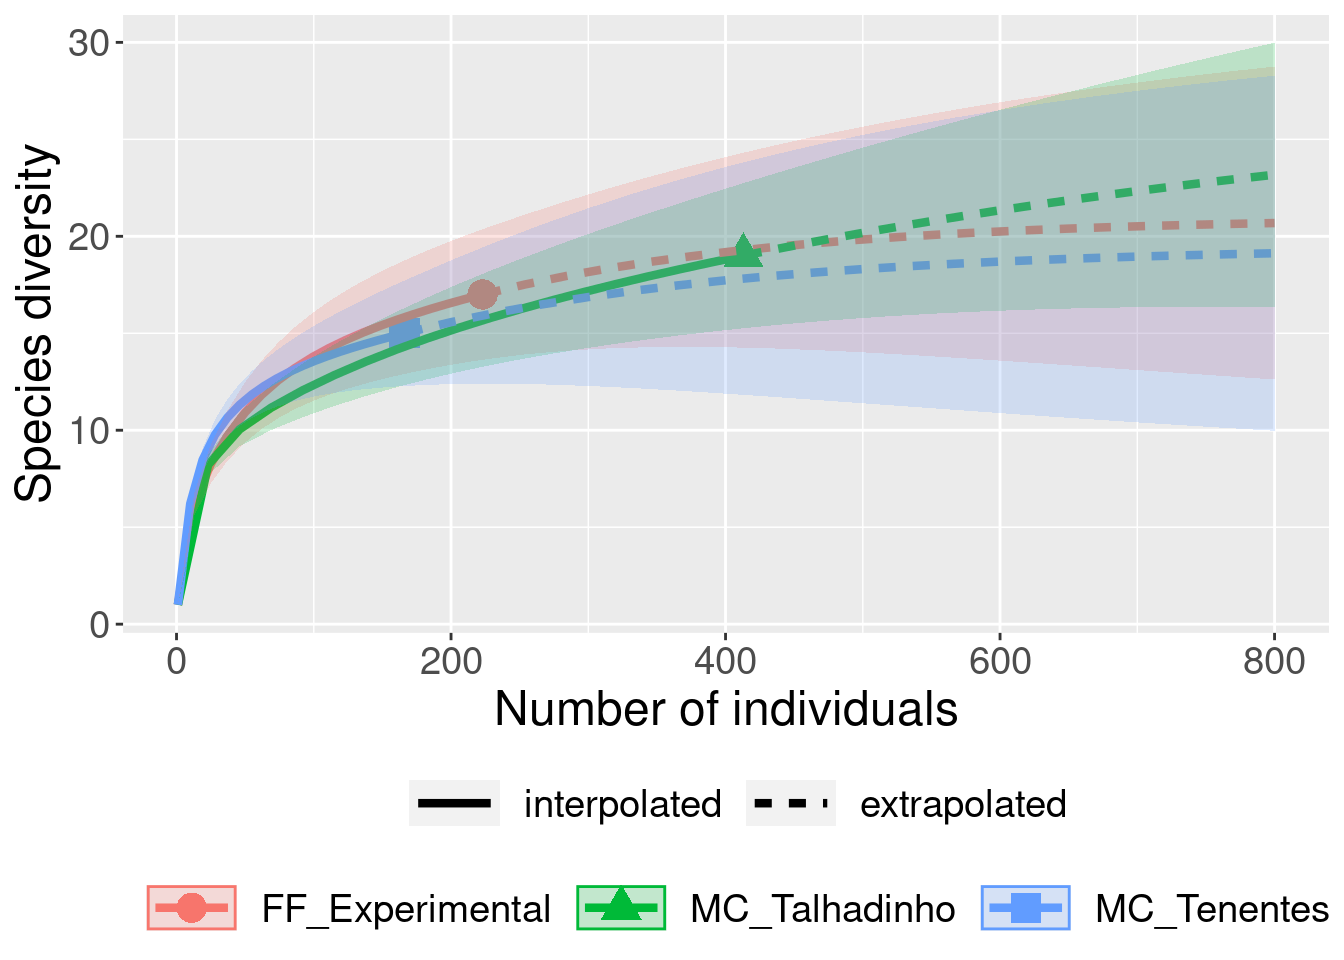
\includegraphics{livro_r_ecologia_files/figure-latex/unnamed-chunk-4-1.pdf}

\textbf{Interpretação dos resultados}

Neste exemplo, foram registrados 166 indivíduos na MC\_Tenentes, 413 na MC\_Talhadinho e 223 na FF\_Experimental. Lembrando, você não pode comparar a riqueza de espécies observada diretamente: 15 espécies na MC\_Tenentes, 17 espécies na MC\_Talhadinho, e 13 espécies no FF\_Experimental. A comparação da riqueza de espécies entre as comunidades deve ser feita com base na riqueza de espécies estimada que é calculada com base no número de indivíduos da comunidade com menor abundância (166 indivíduos). Olhando o gráfico é possível perceber que a riqueza de espécies de morcegos estimada não é diferente entre os três fragmentos florestais quando corrigimos o problema da abundância pela rarefação. A interpretação é feita com base no intervalo de confiança de 95\%. As curvas serão diferentes quando os intervalos de confiança não se sobreporem (Chao et al.~2014). Percebam que está abordagem, além da interpolação (rarefação), também realiza extrapolações que podem ser usadas para estimar o número de espécies caso o esforço de coleta fosse maior. Este é o assunto do nosso próximo tópico.

~

\hypertarget{estimadores-de-riqueza}{%
\chapter{\texorpdfstring{\textbf{Estimadores de riqueza}}{Estimadores de riqueza}}\label{estimadores-de-riqueza}}

\hypertarget{backgorund-da-anuxe1lise-2}{%
\section{Backgorund da análise}\label{backgorund-da-anuxe1lise-2}}

Uma vez que determinar o número total de espécies numa área é praticamente impossível, principalmente em regiões com alta riqueza de espécies, os estimadores são úteis para extrapolar a riqueza observada e tentar estimar a riqueza total através de uma amostra incompleta de uma comunidade biológica (Walther \& Moore 2005). Neste capítulo serão considerados os estimadores não paramétricos que não assumem uma forma de distribuição para a abundância (e.g.~distribuições log-serie ou log-normal), mas usam informações da frequencia de espécies raras na comunidade (Gotelli \& Chao 2013). Para outros estimadores veja Magurran (2004) e Colwell (2019).

\begin{quote}
\hypertarget{quatro-caracteruxedsticas-para-um-bom-estimador-de-riqueza-chazdon-et-al.-1998-horter-et-al.-2006}{%
\subsubsection{Quatro características para um bom estimador de riqueza (Chazdon et al.~1998; Horter et al.~2006):}\label{quatro-caracteruxedsticas-para-um-bom-estimador-de-riqueza-chazdon-et-al.-1998-horter-et-al.-2006}}

\begin{itemize}
\tightlist
\item
  Independência do tamanho da amostra (quantidade de esforço amostral realizado);
\item
  Insensibilidade a diferentes padrões de distribuições (diferentes equitabilidades);
\item
  Insensibilidade em relação à ordem das amostragens;
\item
  Insensibilidade à heterogeneidade entre as amostras usadas entre estudos.
\end{itemize}
\end{quote}

\hypertarget{estimadores-baseados-na-abunduxe2ncia-das-espuxe9cies}{%
\section{\texorpdfstring{\textbf{Estimadores baseados na abundância das espécies}}{Estimadores baseados na abundância das espécies}}\label{estimadores-baseados-na-abunduxe2ncia-das-espuxe9cies}}

\hypertarget{chao-1---chao-1984-1987}{%
\subsection{\texorpdfstring{\textbf{CHAO 1 - (Chao 1984, 1987):}}{CHAO 1 - (Chao 1984, 1987):}}\label{chao-1---chao-1984-1987}}

Estimador simples do número absoluto de espécies em uma comunidade. É baseado no número de espécies raras dentro de uma amostra.

\begin{quote}
\[Chao_{1} = S_{obs} + \left(\frac{n-1}{n}\right)\frac{F_1(F_1-1)}{2(F_2+1)}\]
\end{quote}

onde:

\begin{itemize}
\item
  Sobs = o número de espécies na comunidade,
\item
  \emph{n} = número de amostras,
\item
  F1 = número de espécies observadas com abundância de um indivíduo (espécies \emph{singleton}),
\item
  F2 = número de espécies observadas com abundância de dois indivíduos (espécies \emph{doubletons}).
\end{itemize}

O valor de Chao 1 é máximo quando todas as espécies menos uma são únicas (\emph{singleton}). Neste caso, a riqueza estimada é aproximadamente o dobro da riqueza observada.

~

\hypertarget{exemplo-pruxe1tico---chao-1}{%
\subsubsection{Exemplo prático - Chao 1}\label{exemplo-pruxe1tico---chao-1}}

\hypertarget{explicauxe7uxe3o-dos-dados-1}{%
\paragraph{Explicação dos dados}\label{explicauxe7uxe3o-dos-dados-1}}

Neste exemplo usaremos os dados de 17 espécies de anuros amostradas em 14 dias de coletas de campo em um habitat reprodutivo localizado na região noroeste do estado de São Paulo, Brasil.

\textbf{Pergunta:}

\begin{quote}
Quantas espécies a mais poderiam ser amostradas caso aumentasse o esforço amostral?
\end{quote}

\textbf{Predições}

\begin{quote}
\begin{itemize}
\tightlist
\item
  O número de espécies estimadas é similar ao número de espécies observada;
\item
  O número de espécies estimadas é maior do que o número de espécies observada.
\end{itemize}
\end{quote}

\textbf{Variáveis}

\begin{itemize}
\tightlist
\item
  Variáveis preditoras

  \begin{itemize}
  \tightlist
  \item
    matriz ou vetor com as abundâncias das espécies de anuros registradas em uma habitat reprodutivo
  \end{itemize}
\end{itemize}

\textbf{Checklist}

\begin{itemize}
\tightlist
\item
  Verificar se a sua matriz está com as espécies nas colunas e as amostragens nas linhas
\item
  Verificar se os dados são de abundância e não presença e ausência
\end{itemize}

\hypertarget{anuxe1lise-2}{%
\subsection{Análise}\label{anuxe1lise-2}}

Calculo do estimador de riqueza - Chao 1

\begin{Shaded}
\begin{Highlighting}[]
\KeywordTok{library}\NormalTok{(vegan)}
\NormalTok{dados_coleta <-}\StringTok{ }\NormalTok{poca_anuros}
\NormalTok{est_chao1 <-}\StringTok{ }\KeywordTok{estaccumR}\NormalTok{(dados_coleta, }\DataTypeTok{permutations =} \DecValTok{100}\NormalTok{)}
\end{Highlighting}
\end{Shaded}

\begin{verbatim}
## Warning in sqrt(sum(Deriv.Ch1 %*% t(Deriv.Ch1) * (diag(a) - a %*% t(a)/S.ACE))):
## NaNs produced

## Warning in sqrt(sum(Deriv.Ch1 %*% t(Deriv.Ch1) * (diag(a) - a %*% t(a)/S.ACE))):
## NaNs produced

## Warning in sqrt(sum(Deriv.Ch1 %*% t(Deriv.Ch1) * (diag(a) - a %*% t(a)/S.ACE))):
## NaNs produced

## Warning in sqrt(sum(Deriv.Ch1 %*% t(Deriv.Ch1) * (diag(a) - a %*% t(a)/S.ACE))):
## NaNs produced

## Warning in sqrt(sum(Deriv.Ch1 %*% t(Deriv.Ch1) * (diag(a) - a %*% t(a)/S.ACE))):
## NaNs produced

## Warning in sqrt(sum(Deriv.Ch1 %*% t(Deriv.Ch1) * (diag(a) - a %*% t(a)/S.ACE))):
## NaNs produced

## Warning in sqrt(sum(Deriv.Ch1 %*% t(Deriv.Ch1) * (diag(a) - a %*% t(a)/S.ACE))):
## NaNs produced
\end{verbatim}

\begin{Shaded}
\begin{Highlighting}[]
\KeywordTok{summary}\NormalTok{(est_chao1, }\DataTypeTok{display =} \StringTok{"chao"}\NormalTok{)}
\end{Highlighting}
\end{Shaded}

\begin{verbatim}
## $chao
##         N      Chao   2.5%    97.5%  Std.Dev
## Dia_8   1  6.324167  3.000 12.33333 2.784056
## Dia_2   2  9.684167  6.000 17.50000 3.250578
## Dia_6   3 11.287333  6.000 17.52500 2.872768
## Dia_3   4 12.191667  7.475 17.70000 2.474718
## Dia_10  5 13.305833  9.000 19.52500 2.593349
## Dia_5   6 14.256667 10.000 22.00000 2.987574
## Dia_9   7 14.990000 11.000 22.00000 2.710169
## Dia_4   8 15.918333 11.475 22.00000 2.753377
## Dia_11  9 16.638333 12.475 22.00000 2.688573
## Dia_12 10 17.248333 13.000 22.00000 2.756433
## Dia_13 11 18.305000 14.000 22.00000 2.479100
## Dia_14 12 19.030000 14.975 22.00000 2.110364
## Dia_1  13 19.460000 15.500 22.00000 1.569404
## Dia_7  14 20.000000 20.000 20.00000 0.000000
## 
## attr(,"class")
## [1] "summary.poolaccum"
\end{verbatim}

Visualizar os resultados com intervalo de confiança de 95\%.

\begin{Shaded}
\begin{Highlighting}[]
\KeywordTok{library}\NormalTok{(ggplot2)}
\CommentTok{# preparando os dados para fazer o gráfico}
\NormalTok{resultados <-}\StringTok{ }\KeywordTok{summary}\NormalTok{(est_chao1, }\DataTypeTok{display =} \KeywordTok{c}\NormalTok{(}\StringTok{"S"}\NormalTok{, }\StringTok{"chao"}\NormalTok{))}
\NormalTok{res_chao <-}\StringTok{ }\KeywordTok{cbind}\NormalTok{(resultados}\OperatorTok{$}\NormalTok{chao[,}\DecValTok{1}\OperatorTok{:}\DecValTok{4}\NormalTok{], resultados}\OperatorTok{$}\NormalTok{S[,}\DecValTok{2}\OperatorTok{:}\DecValTok{4}\NormalTok{])}
\NormalTok{res_chao <-}\StringTok{ }\KeywordTok{as.data.frame}\NormalTok{(res_chao)}
\KeywordTok{colnames}\NormalTok{(res_chao) <-}\StringTok{ }\KeywordTok{c}\NormalTok{(}\StringTok{"Amostras"}\NormalTok{, }\StringTok{"Chao"}\NormalTok{, }\StringTok{"C_inferior"}\NormalTok{, }\StringTok{"C_superior"}\NormalTok{, }\StringTok{"Riqueza"}\NormalTok{,}
                        \StringTok{"R_inferior"}\NormalTok{, }\StringTok{"R_superior"}\NormalTok{)}

\CommentTok{# comando para o gráfico}
\KeywordTok{ggplot}\NormalTok{(res_chao, }\KeywordTok{aes}\NormalTok{(}\DataTypeTok{y =}\NormalTok{ Riqueza, }\DataTypeTok{x =}\NormalTok{ Amostras)) }\OperatorTok{+}
\StringTok{  }\KeywordTok{geom_point}\NormalTok{(}\KeywordTok{aes}\NormalTok{(}\DataTypeTok{y =}\NormalTok{ Chao, }\DataTypeTok{x =}\NormalTok{ Amostras }\OperatorTok{+}\StringTok{ }\FloatTok{0.1}\NormalTok{), }\DataTypeTok{size =} \DecValTok{5}\NormalTok{, }\DataTypeTok{color =} \StringTok{"blue"}\NormalTok{, }\DataTypeTok{alpha =} \DecValTok{1}\NormalTok{) }\OperatorTok{+}
\StringTok{  }\KeywordTok{geom_point}\NormalTok{(}\KeywordTok{aes}\NormalTok{(}\DataTypeTok{y =}\NormalTok{ Riqueza, }\DataTypeTok{x =}\NormalTok{ Amostras), }\DataTypeTok{size =} \DecValTok{5}\NormalTok{, }\DataTypeTok{color =} \StringTok{"red"}\NormalTok{, }\DataTypeTok{alpha =} \DecValTok{1}\NormalTok{) }\OperatorTok{+}
\StringTok{  }\KeywordTok{geom_line}\NormalTok{ (}\KeywordTok{aes}\NormalTok{(}\DataTypeTok{y =}\NormalTok{ Chao, }\DataTypeTok{x =}\NormalTok{ Amostras), }\DataTypeTok{color =} \StringTok{"blue"}\NormalTok{) }\OperatorTok{+}
\StringTok{  }\KeywordTok{geom_line}\NormalTok{ (}\KeywordTok{aes}\NormalTok{(}\DataTypeTok{y =}\NormalTok{ Riqueza, }\DataTypeTok{x =}\NormalTok{ Amostras), }\DataTypeTok{color =} \StringTok{"red"}\NormalTok{) }\OperatorTok{+}
\StringTok{  }\KeywordTok{geom_linerange}\NormalTok{(}\KeywordTok{aes}\NormalTok{(}\DataTypeTok{ymin =}\NormalTok{ C_inferior, }\DataTypeTok{ymax =}\NormalTok{ C_superior, }\DataTypeTok{x =}\NormalTok{ Amostras }\OperatorTok{+}\StringTok{ }\FloatTok{0.1}\NormalTok{),}
 \DataTypeTok{color =} \StringTok{"blue"}\NormalTok{) }\OperatorTok{+}
\StringTok{  }\KeywordTok{geom_linerange}\NormalTok{(}\KeywordTok{aes}\NormalTok{(}\DataTypeTok{ymin =}\NormalTok{ R_inferior, }\DataTypeTok{ymax =}\NormalTok{ R_superior, }\DataTypeTok{x =}\NormalTok{ Amostras), }\DataTypeTok{color =} \StringTok{"red"}\NormalTok{) }\OperatorTok{+}
\StringTok{  }\KeywordTok{ylab}\NormalTok{ (}\StringTok{"Estimador de riqueza - Chao 1"}\NormalTok{) }\OperatorTok{+}
\StringTok{  }\KeywordTok{xlab}\NormalTok{ (}\StringTok{"Número de amostras"}\NormalTok{) }\OperatorTok{+}
\StringTok{  }\KeywordTok{scale_x_continuous}\NormalTok{(}\DataTypeTok{limits =} \KeywordTok{c}\NormalTok{(}\DecValTok{1}\NormalTok{,}\DecValTok{15}\NormalTok{), }\DataTypeTok{breaks=}\KeywordTok{seq}\NormalTok{(}\DecValTok{1}\NormalTok{,}\DecValTok{15}\NormalTok{,}\DecValTok{1}\NormalTok{)) }\OperatorTok{+}
\StringTok{  }\KeywordTok{geom_point}\NormalTok{(}\DataTypeTok{y=} \FloatTok{7.5}\NormalTok{, }\DataTypeTok{x =} \DecValTok{9}\NormalTok{, }\DataTypeTok{size =} \DecValTok{5}\NormalTok{, }\DataTypeTok{color =} \StringTok{"blue"}\NormalTok{, }\DataTypeTok{alpha =} \DecValTok{1}\NormalTok{) }\OperatorTok{+}\StringTok{ }
\StringTok{  }\KeywordTok{geom_point}\NormalTok{(}\DataTypeTok{y=} \FloatTok{5.9}\NormalTok{, }\DataTypeTok{x =} \DecValTok{9}\NormalTok{, }\DataTypeTok{size =} \DecValTok{5}\NormalTok{, }\DataTypeTok{color =} \StringTok{"red"}\NormalTok{, }\DataTypeTok{alpha =} \DecValTok{1}\NormalTok{) }\OperatorTok{+}\StringTok{ }
\StringTok{  }\KeywordTok{geom_label}\NormalTok{( }\DataTypeTok{y =} \FloatTok{7.5}\NormalTok{, }\DataTypeTok{x =} \DecValTok{12}\NormalTok{, }\DataTypeTok{label =} \StringTok{"Riqueza estimada - Chao 1"}\NormalTok{) }\OperatorTok{+}
\StringTok{  }\KeywordTok{geom_label}\NormalTok{( }\DataTypeTok{y =} \FloatTok{5.9}\NormalTok{, }\DataTypeTok{x =} \FloatTok{11.3}\NormalTok{, }\DataTypeTok{label =} \StringTok{"Riqueza observada"}\NormalTok{)}
\end{Highlighting}
\end{Shaded}

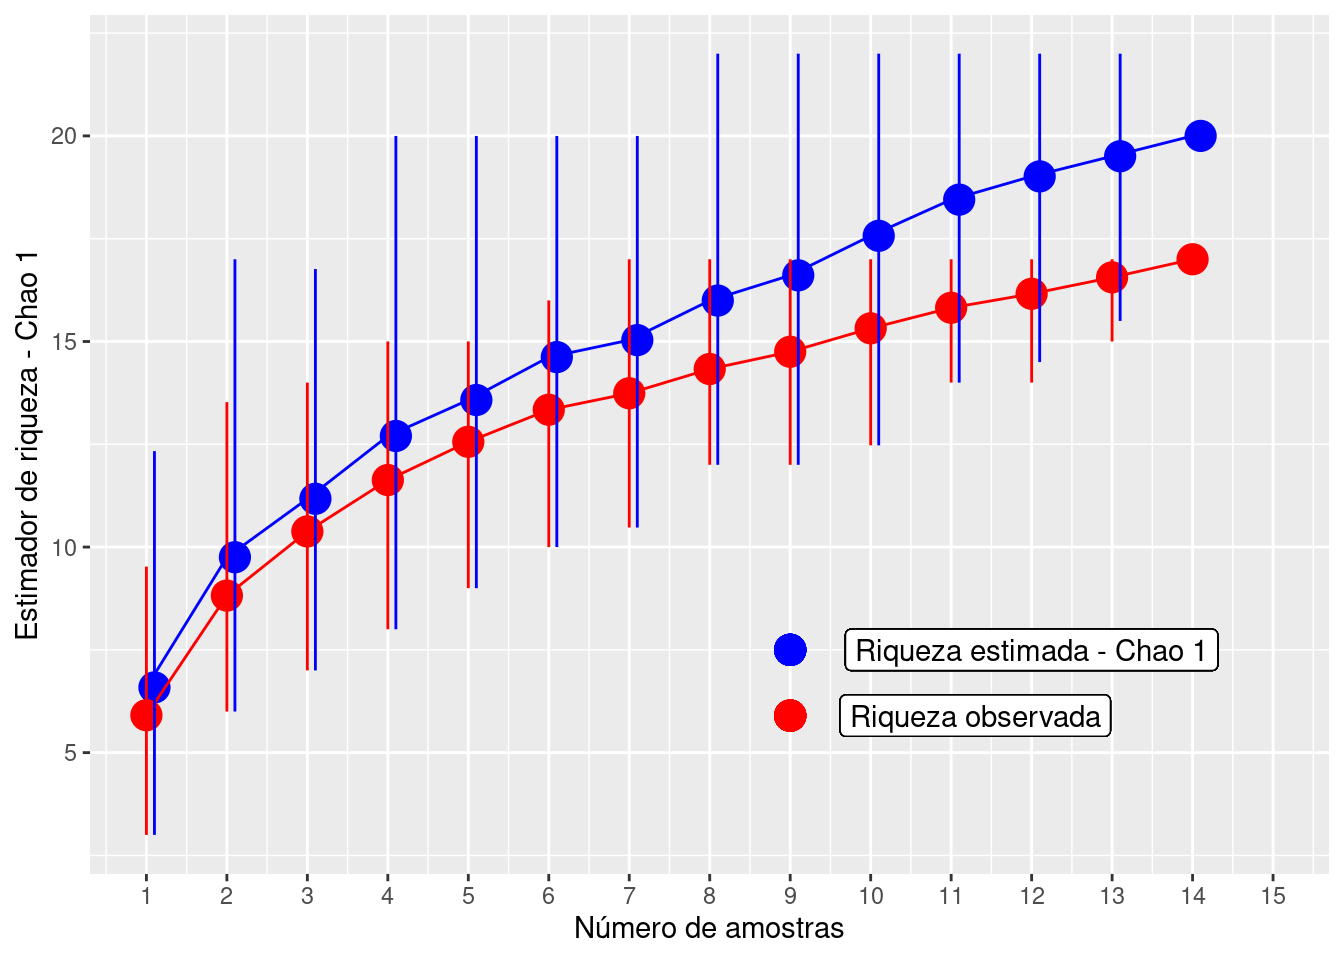
\includegraphics{livro_r_ecologia_files/figure-latex/unnamed-chunk-6-1.pdf}

\hypertarget{interpretauxe7uxe3o-dos-resultados-1}{%
\subsubsection{Interpretação dos resultados}\label{interpretauxe7uxe3o-dos-resultados-1}}

Com base no número de espécies raras (\emph{singletons} e \emph{doubletons}), o estimador Chao 1 indica a possibilidade de encontrarmos mais três espécies caso o esforço amostral fosse maior e não mostra tendência de estabilização da curva em uma assíntota.

\hypertarget{ace---abundance-based-coverage-estimador-chao-lee-1992-chao-et-al.-2000}{%
\subsection{\texorpdfstring{\textbf{ACE - \emph{Abundance-based Coverage Estimador} (Chao \& Lee 1992, Chao et al.~2000):}}{ACE - Abundance-based Coverage Estimador (Chao \& Lee 1992, Chao et al.~2000):}}\label{ace---abundance-based-coverage-estimador-chao-lee-1992-chao-et-al.-2000}}

Este método trabalha com a abundância das espécies raras (i.e.~abundância baixa). Entretanto, diferente do estimador anterior, esse método permite ao pesquisador determinar os limites para os quais uma espécie seja considerada rara. Em geral, são consideradas raras espécies com abundância entre 1 e 10 indivíduos. A riqueza estimada pode variar conforme se aumente ou diminua o limiar de abundância, e infelizmente não existem critérios biológicos definidos para a escolha do melhor intervalo.

\begin{quote}
\[ACE = S_{abund} + \frac{S_{rare}}{C_{ace}} + \frac{F_1}{C_{ace}}Y_{ace}^2\]
\end{quote}

onde:

\begin{quote}
\[Y_{ace}^2 = max \left[\frac{S_{rare}}{C_{ace}}\frac{\sum_{i=i}^{10}i(i-1)F1}{(N_{rare})({N_{rare} - 1)}}-1,0\right]\]
\end{quote}

\begin{quote}
\[C_{ace} = 1 - \frac{F1}{N_{rare}}\]
\end{quote}

\begin{quote}
\[N_{rare} = \sum_{i=1}^{10}iF_i\]
\end{quote}

Não precisa fazer cara feia, é óbvio que iremos usar o programa para fazer esses cálculos.

~

\hypertarget{exemplo-pruxe1tico---ace}{%
\subsubsection{Exemplo prático - ACE}\label{exemplo-pruxe1tico---ace}}

\hypertarget{explicauxe7uxe3o-dos-dados-2}{%
\paragraph{Explicação dos dados}\label{explicauxe7uxe3o-dos-dados-2}}

Usaremos os mesmos dados de 17 espécies de anuros amostradas em 14 dias de coletas de campo em um habitat reprodutivo localizado na região noroeste do estado de São Paulo, Brasil.

\textbf{Pergunta:}

\begin{quote}
Quantas espécies a mais poderiam ser amostradas caso aumentasse o esforço amostral?
\end{quote}

\textbf{Predições}

\begin{quote}
\begin{itemize}
\tightlist
\item
  O número de espécies estimadas é similar ao número de espécies observada;
\item
  O número de espécies estimadas é maior do que o número de espécies observada.
\end{itemize}
\end{quote}

\textbf{Variáveis}

\begin{itemize}
\tightlist
\item
  Variáveis preditoras

  \begin{itemize}
  \tightlist
  \item
    matriz ou vetor com as abundâncias das espécies de anuros registradas em uma habitat reprodutivo
  \end{itemize}
\end{itemize}

\textbf{Checklist}

\begin{itemize}
\tightlist
\item
  Verificar se a sua matriz está com as espécies nas colunas e as amostragens nas linhas
\item
  Verificar se os dados são de abundância e não presença e ausência
\end{itemize}

\hypertarget{anuxe1lise-3}{%
\subsection{Análise}\label{anuxe1lise-3}}

Calculo do estimador de riqueza - ACE

\begin{Shaded}
\begin{Highlighting}[]
\KeywordTok{library}\NormalTok{(vegan)}
\NormalTok{dados_coleta <-}\StringTok{ }\NormalTok{poca_anuros}
\NormalTok{est_ace <-}\StringTok{ }\KeywordTok{estaccumR}\NormalTok{(dados_coleta, }\DataTypeTok{permutations =} \DecValTok{100}\NormalTok{)}
\end{Highlighting}
\end{Shaded}

\begin{verbatim}
## Warning in sqrt(sum(Deriv.Ch1 %*% t(Deriv.Ch1) * (diag(a) - a %*% t(a)/S.ACE))):
## NaNs produced

## Warning in sqrt(sum(Deriv.Ch1 %*% t(Deriv.Ch1) * (diag(a) - a %*% t(a)/S.ACE))):
## NaNs produced

## Warning in sqrt(sum(Deriv.Ch1 %*% t(Deriv.Ch1) * (diag(a) - a %*% t(a)/S.ACE))):
## NaNs produced

## Warning in sqrt(sum(Deriv.Ch1 %*% t(Deriv.Ch1) * (diag(a) - a %*% t(a)/S.ACE))):
## NaNs produced

## Warning in sqrt(sum(Deriv.Ch1 %*% t(Deriv.Ch1) * (diag(a) - a %*% t(a)/S.ACE))):
## NaNs produced
\end{verbatim}

\begin{Shaded}
\begin{Highlighting}[]
\KeywordTok{summary}\NormalTok{(est_ace, }\DataTypeTok{display =} \StringTok{"ace"}\NormalTok{)}
\end{Highlighting}
\end{Shaded}

\begin{verbatim}
## $ace
##         N       ACE      2.5%    97.5%  Std.Dev
## Dia_10  1  7.312599  3.545190 13.71429 2.507754
## Dia_6   2  9.867772  6.000000 15.32094 2.615741
## Dia_3   3 11.381572  8.000000 15.74236 2.196049
## Dia_12  4 12.309283  8.121225 18.30396 2.521721
## Dia_11  5 13.254672  9.300926 17.83543 2.373748
## Dia_14  6 13.962945 10.000000 20.09544 2.612751
## Dia_8   7 14.772572 10.000000 20.81838 2.597293
## Dia_5   8 16.126711 11.000000 22.86709 3.142946
## Dia_4   9 17.406325 12.000000 24.44538 3.496535
## Dia_13 10 19.099780 12.708320 25.72368 3.777796
## Dia_7  11 21.150317 13.720826 25.72368 3.797767
## Dia_9  12 22.617325 16.401709 25.72368 3.258174
## Dia_2  13 23.781985 17.676471 25.72368 2.337662
## Dia_1  14 24.703704 24.703704 24.70370 0.000000
## 
## attr(,"class")
## [1] "summary.poolaccum"
\end{verbatim}

Visualizar os resultados com intervalo de confiança de 95\%

\begin{Shaded}
\begin{Highlighting}[]
\KeywordTok{library}\NormalTok{(ggplot2)}
\CommentTok{# preparando os dados para fazer o gráfico}
\NormalTok{resultados_ace <-}\StringTok{ }\KeywordTok{summary}\NormalTok{(est_ace, }\DataTypeTok{display =} \KeywordTok{c}\NormalTok{(}\StringTok{"S"}\NormalTok{, }\StringTok{"ace"}\NormalTok{))}
\NormalTok{res_ace <-}\StringTok{ }\KeywordTok{cbind}\NormalTok{(resultados_ace}\OperatorTok{$}\NormalTok{ace[,}\DecValTok{1}\OperatorTok{:}\DecValTok{4}\NormalTok{], resultados_ace}\OperatorTok{$}\NormalTok{S[,}\DecValTok{2}\OperatorTok{:}\DecValTok{4}\NormalTok{])}
\NormalTok{res_ace <-}\StringTok{ }\KeywordTok{as.data.frame}\NormalTok{(res_ace)}
\KeywordTok{colnames}\NormalTok{(res_ace) <-}\StringTok{ }\KeywordTok{c}\NormalTok{(}\StringTok{"Amostras"}\NormalTok{, }\StringTok{"ACE"}\NormalTok{, }\StringTok{"ACE_inferior"}\NormalTok{, }\StringTok{"ACE_superior"}\NormalTok{, }\StringTok{"Riqueza"}\NormalTok{,}
                        \StringTok{"R_inferior"}\NormalTok{, }\StringTok{"R_superior"}\NormalTok{)}

\CommentTok{# comando para o gráfico}
\KeywordTok{ggplot}\NormalTok{(res_ace, }\KeywordTok{aes}\NormalTok{(}\DataTypeTok{y =}\NormalTok{ Riqueza, }\DataTypeTok{x =}\NormalTok{ Amostras)) }\OperatorTok{+}
\StringTok{  }\KeywordTok{geom_point}\NormalTok{(}\KeywordTok{aes}\NormalTok{(}\DataTypeTok{y =}\NormalTok{ ACE, }\DataTypeTok{x =}\NormalTok{ Amostras }\OperatorTok{+}\StringTok{ }\FloatTok{0.1}\NormalTok{), }\DataTypeTok{size =} \DecValTok{5}\NormalTok{, }\DataTypeTok{color =} \StringTok{"blue"}\NormalTok{, }\DataTypeTok{alpha =} \DecValTok{1}\NormalTok{) }\OperatorTok{+}
\StringTok{  }\KeywordTok{geom_point}\NormalTok{(}\KeywordTok{aes}\NormalTok{(}\DataTypeTok{y =}\NormalTok{ Riqueza, }\DataTypeTok{x =}\NormalTok{ Amostras), }\DataTypeTok{size =} \DecValTok{5}\NormalTok{, }\DataTypeTok{color =} \StringTok{"red"}\NormalTok{, }\DataTypeTok{alpha =} \DecValTok{1}\NormalTok{) }\OperatorTok{+}
\StringTok{  }\KeywordTok{geom_line}\NormalTok{ (}\KeywordTok{aes}\NormalTok{(}\DataTypeTok{y =}\NormalTok{ ACE, }\DataTypeTok{x =}\NormalTok{ Amostras), }\DataTypeTok{color =} \StringTok{"blue"}\NormalTok{) }\OperatorTok{+}
\StringTok{  }\KeywordTok{geom_line}\NormalTok{ (}\KeywordTok{aes}\NormalTok{(}\DataTypeTok{y =}\NormalTok{ Riqueza, }\DataTypeTok{x =}\NormalTok{ Amostras), }\DataTypeTok{color =} \StringTok{"red"}\NormalTok{) }\OperatorTok{+}
\StringTok{  }\KeywordTok{geom_linerange}\NormalTok{(}\KeywordTok{aes}\NormalTok{(}\DataTypeTok{ymin =}\NormalTok{ ACE_inferior, }\DataTypeTok{ymax =}\NormalTok{ ACE_superior, }\DataTypeTok{x =}\NormalTok{ Amostras }\OperatorTok{+}\StringTok{ }\FloatTok{0.1}\NormalTok{),}
 \DataTypeTok{color =} \StringTok{"blue"}\NormalTok{) }\OperatorTok{+}
\StringTok{  }\KeywordTok{geom_linerange}\NormalTok{(}\KeywordTok{aes}\NormalTok{(}\DataTypeTok{ymin =}\NormalTok{ R_inferior, }\DataTypeTok{ymax =}\NormalTok{ R_superior, }\DataTypeTok{x =}\NormalTok{ Amostras), }\DataTypeTok{color =} \StringTok{"red"}\NormalTok{) }\OperatorTok{+}
\StringTok{  }\KeywordTok{ylab}\NormalTok{ (}\StringTok{"Estimador de riqueza - ACE"}\NormalTok{) }\OperatorTok{+}
\StringTok{  }\KeywordTok{xlab}\NormalTok{ (}\StringTok{"Número de amostras"}\NormalTok{) }\OperatorTok{+}
\StringTok{  }\KeywordTok{scale_x_continuous}\NormalTok{(}\DataTypeTok{limits =} \KeywordTok{c}\NormalTok{(}\DecValTok{1}\NormalTok{,}\DecValTok{15}\NormalTok{), }\DataTypeTok{breaks=}\KeywordTok{seq}\NormalTok{(}\DecValTok{1}\NormalTok{,}\DecValTok{15}\NormalTok{,}\DecValTok{1}\NormalTok{)) }\OperatorTok{+}
\StringTok{  }\KeywordTok{geom_point}\NormalTok{(}\DataTypeTok{y=} \FloatTok{7.5}\NormalTok{, }\DataTypeTok{x =} \DecValTok{9}\NormalTok{, }\DataTypeTok{size =} \DecValTok{5}\NormalTok{, }\DataTypeTok{color =} \StringTok{"blue"}\NormalTok{, }\DataTypeTok{alpha =} \DecValTok{1}\NormalTok{) }\OperatorTok{+}\StringTok{ }
\StringTok{  }\KeywordTok{geom_point}\NormalTok{(}\DataTypeTok{y=} \FloatTok{5.9}\NormalTok{, }\DataTypeTok{x =} \DecValTok{9}\NormalTok{, }\DataTypeTok{size =} \DecValTok{5}\NormalTok{, }\DataTypeTok{color =} \StringTok{"red"}\NormalTok{, }\DataTypeTok{alpha =} \DecValTok{1}\NormalTok{) }\OperatorTok{+}\StringTok{ }
\StringTok{  }\KeywordTok{geom_label}\NormalTok{( }\DataTypeTok{y =} \FloatTok{7.5}\NormalTok{, }\DataTypeTok{x =} \FloatTok{11.7}\NormalTok{, }\DataTypeTok{label =} \StringTok{"Riqueza estimada - ACE"}\NormalTok{) }\OperatorTok{+}
\StringTok{  }\KeywordTok{geom_label}\NormalTok{( }\DataTypeTok{y =} \FloatTok{5.9}\NormalTok{, }\DataTypeTok{x =} \FloatTok{11.3}\NormalTok{, }\DataTypeTok{label =} \StringTok{"Riqueza observada"}\NormalTok{)}
\end{Highlighting}
\end{Shaded}

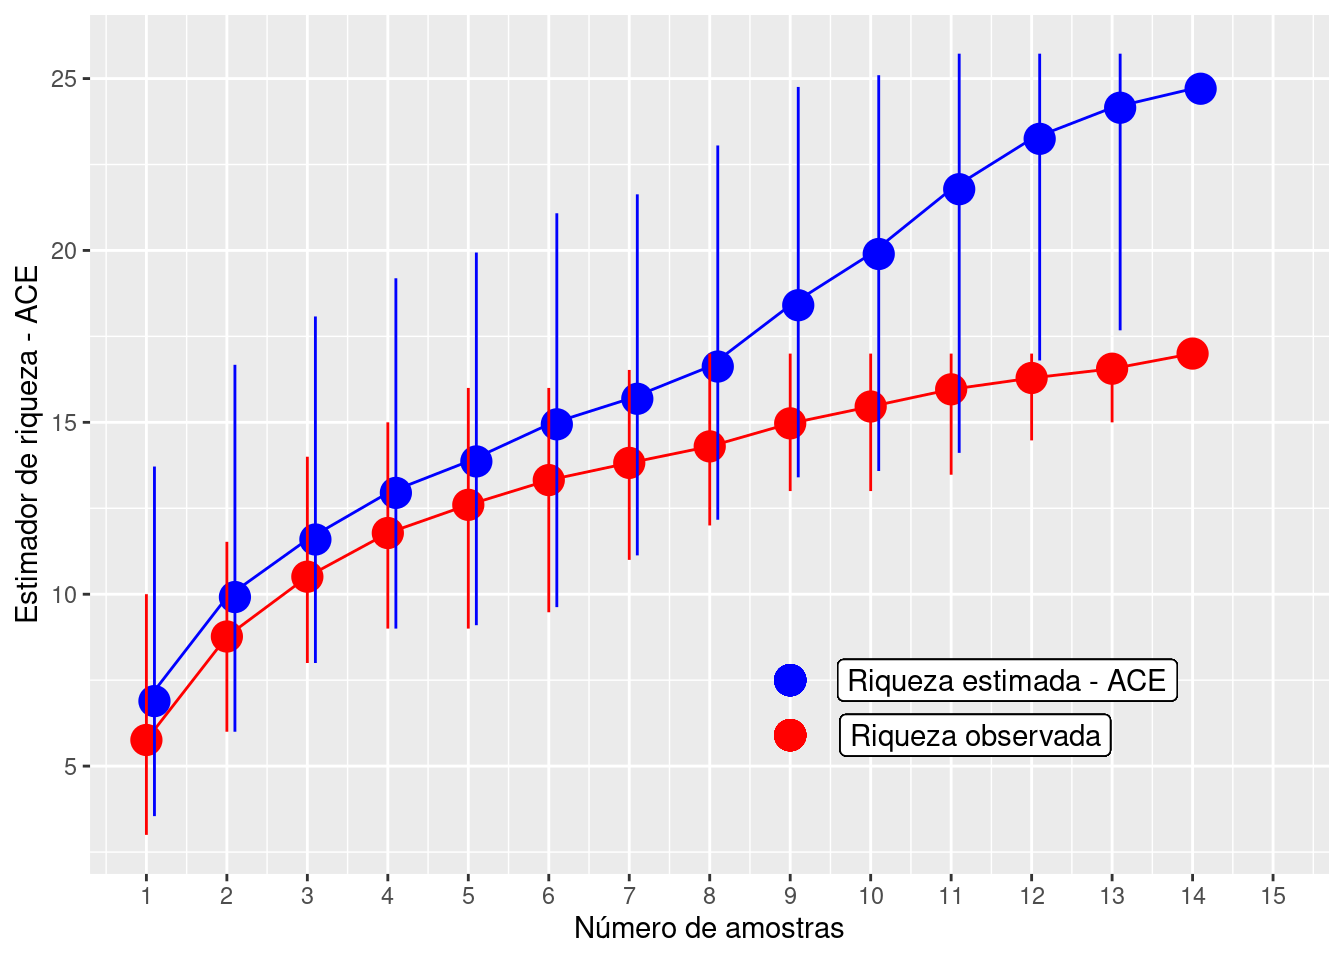
\includegraphics{livro_r_ecologia_files/figure-latex/unnamed-chunk-8-1.pdf}

\hypertarget{interpretauxe7uxe3o-dos-resultados-2}{%
\subsubsection{Interpretação dos resultados}\label{interpretauxe7uxe3o-dos-resultados-2}}

Com base no número de espécies raras (abundância menor que 10 indivíduos - \emph{default}), o estimador ACE indica a possibilidade de encontrarmos mais sete espécies caso o esforço amostral fosse maior e não mostrou tendência de estabilição da curva em uma assíntota.

\hypertarget{estimadores-baseados-na-inciduxeancia-das-espuxe9cies}{%
\section{\texorpdfstring{\textbf{Estimadores baseados na incidência das espécies}}{Estimadores baseados na incidência das espécies}}\label{estimadores-baseados-na-inciduxeancia-das-espuxe9cies}}

\hypertarget{chao-2---chao-1987}{%
\subsection{\texorpdfstring{\textbf{CHAO 2 - (Chao 1987):}}{CHAO 2 - (Chao 1987):}}\label{chao-2---chao-1987}}

De acordo com Anne Chao, o estimador Chao 1 pode ser modificado para uso com dados de presença/ausência levando em conta a distribuição das espécies entre amostras. Neste caso é
necessário somente conhecer o número de espécies encontradas em somente uma amostra e o
número de espécies encontradas exatamente em duas amostras. Essa variação ficou denominada como
Chao 2:

\begin{quote}
\[Chao_{2} = S_{obs} + \left(\frac{m-1}{m}\right)\left(\frac{Q_1(Q_1-1)}{2(Q_2 + 1}\right)\]
\end{quote}

onde:

\begin{itemize}
\item
  Sobs = o número de espécies na comunidade,
\item
  \emph{m} = número de amostragens,
\item
  Q1 = número de espécies observadas em uma amostragem (espécies \emph{uniques}),
\item
  Q2 = número de espécies observadas em duas amostragens (espécies \emph{duplicates}).
\end{itemize}

O valor de Chao2 é máximo quando as espécies menos uma são únicas (\emph{uniques}). Neste caso, a riqueza estimada é aproximadamente o dobro da riqueza observada. Colwell \& Coddington (1994) encontraram que o valor de Chao 2 mostrou ser o estimador menos enviesado para amostras com tamanho pequeno.

~

\hypertarget{exemplo-pruxe1tico---chao-2}{%
\subsubsection{Exemplo prático - Chao 2}\label{exemplo-pruxe1tico---chao-2}}

\hypertarget{explicauxe7uxe3o-dos-dados-3}{%
\paragraph{Explicação dos dados}\label{explicauxe7uxe3o-dos-dados-3}}

Usaremos os mesmos dados de 17 espécies de anuros amostradas em 14 dias de coletas de campo em um habitat reprodutivo localizado na região noroeste do estado de São Paulo, Brasil.

\textbf{Pergunta:}

\begin{quote}
Quantas espécies a mais poderiam ser amostradas caso aumentasse o esforço amostral?
\end{quote}

\textbf{Predições}

\begin{quote}
\begin{itemize}
\tightlist
\item
  O número de espécies estimadas é similar ao número de espécies observada;
\item
  O número de espécies estimadas é maior do que o número de espécies observada.
\end{itemize}
\end{quote}

\textbf{Variáveis}

\begin{itemize}
\tightlist
\item
  Variáveis preditoras

  \begin{itemize}
  \tightlist
  \item
    matriz ou vetor com a incidência das espécies de anuros registradas em uma habitat reprodutivo
  \end{itemize}
\end{itemize}

\textbf{Checklist}

\begin{itemize}
\tightlist
\item
  Verificar se a sua matriz está com as espécies nas colunas e as amostragens nas linhas
\end{itemize}

\hypertarget{anuxe1lise-4}{%
\subsection{Análise}\label{anuxe1lise-4}}

Calculo do estimador de riqueza - Chao 2

\begin{Shaded}
\begin{Highlighting}[]
\KeywordTok{library}\NormalTok{(vegan)}
\NormalTok{dados_coleta <-}\StringTok{ }\NormalTok{poca_anuros}
\NormalTok{est_chao2 <-}\StringTok{ }\KeywordTok{poolaccum}\NormalTok{(dados_coleta, }\DataTypeTok{permutations =} \DecValTok{100}\NormalTok{)}
\KeywordTok{summary}\NormalTok{(est_chao2, }\DataTypeTok{display =} \StringTok{"chao"}\NormalTok{)}
\end{Highlighting}
\end{Shaded}

\begin{verbatim}
## $chao
##        N     Chao      2.5%    97.5%  Std.Dev
##  [1,]  3 15.02880  9.105556 22.84167 4.505630
##  [2,]  4 15.09276  9.093750 26.02500 4.656514
##  [3,]  5 17.02633 11.130000 39.08000 6.470241
##  [4,]  6 18.64104 11.336806 36.41667 7.081526
##  [5,]  7 20.17414 11.857143 37.00000 6.508327
##  [6,]  8 21.68740 12.471094 34.37500 6.536800
##  [7,]  9 23.51111 12.888889 40.41111 7.451675
##  [8,] 10 25.30400 14.280000 40.70375 7.450279
##  [9,] 11 27.67091 15.401136 39.27273 6.936816
## [10,] 12 29.79104 18.125000 39.45833 6.424517
## [11,] 13 31.17077 22.384615 39.61538 4.797153
## [12,] 14 33.71429 33.714286 33.71429 0.000000
## 
## attr(,"class")
## [1] "summary.poolaccum"
\end{verbatim}

Visualizar os resultados com intervalo de confiança de 95\%

\begin{Shaded}
\begin{Highlighting}[]
\KeywordTok{library}\NormalTok{(ggplot2)}
\CommentTok{# preparando os dados para fazer o gráfico}
\NormalTok{resultados_chao2 <-}\StringTok{ }\KeywordTok{summary}\NormalTok{(est_chao2, }\DataTypeTok{display =} \KeywordTok{c}\NormalTok{(}\StringTok{"S"}\NormalTok{, }\StringTok{"chao"}\NormalTok{))}
\NormalTok{res_chao2 <-}\StringTok{ }\KeywordTok{cbind}\NormalTok{(resultados_chao2}\OperatorTok{$}\NormalTok{chao[,}\DecValTok{1}\OperatorTok{:}\DecValTok{4}\NormalTok{], resultados_chao2}\OperatorTok{$}\NormalTok{S[,}\DecValTok{2}\OperatorTok{:}\DecValTok{4}\NormalTok{])}
\NormalTok{res_chao2 <-}\StringTok{ }\KeywordTok{as.data.frame}\NormalTok{(res_chao2)}
\KeywordTok{colnames}\NormalTok{(res_chao2) <-}\StringTok{ }\KeywordTok{c}\NormalTok{(}\StringTok{"Amostras"}\NormalTok{, }\StringTok{"Chao2"}\NormalTok{, }\StringTok{"C_inferior"}\NormalTok{, }\StringTok{"C_superior"}\NormalTok{, }\StringTok{"Riqueza"}\NormalTok{,}
                        \StringTok{"R_inferior"}\NormalTok{, }\StringTok{"R_superior"}\NormalTok{)}

\CommentTok{# comando para o gráfico}
\KeywordTok{ggplot}\NormalTok{(res_chao2, }\KeywordTok{aes}\NormalTok{(}\DataTypeTok{y =}\NormalTok{ Riqueza, }\DataTypeTok{x =}\NormalTok{ Amostras)) }\OperatorTok{+}
\StringTok{  }\KeywordTok{geom_point}\NormalTok{(}\KeywordTok{aes}\NormalTok{(}\DataTypeTok{y =}\NormalTok{ Chao2, }\DataTypeTok{x =}\NormalTok{ Amostras }\OperatorTok{+}\StringTok{ }\FloatTok{0.1}\NormalTok{), }\DataTypeTok{size =} \DecValTok{5}\NormalTok{, }\DataTypeTok{color =} \StringTok{"blue"}\NormalTok{, }\DataTypeTok{alpha =} \DecValTok{1}\NormalTok{) }\OperatorTok{+}
\StringTok{  }\KeywordTok{geom_point}\NormalTok{(}\KeywordTok{aes}\NormalTok{(}\DataTypeTok{y =}\NormalTok{ Riqueza, }\DataTypeTok{x =}\NormalTok{ Amostras), }\DataTypeTok{size =} \DecValTok{5}\NormalTok{, }\DataTypeTok{color =} \StringTok{"red"}\NormalTok{, }\DataTypeTok{alpha =} \DecValTok{1}\NormalTok{) }\OperatorTok{+}
\StringTok{  }\KeywordTok{geom_line}\NormalTok{ (}\KeywordTok{aes}\NormalTok{(}\DataTypeTok{y =}\NormalTok{ Chao2, }\DataTypeTok{x =}\NormalTok{ Amostras), }\DataTypeTok{color =} \StringTok{"blue"}\NormalTok{) }\OperatorTok{+}
\StringTok{  }\KeywordTok{geom_line}\NormalTok{ (}\KeywordTok{aes}\NormalTok{(}\DataTypeTok{y =}\NormalTok{ Riqueza, }\DataTypeTok{x =}\NormalTok{ Amostras), }\DataTypeTok{color =} \StringTok{"red"}\NormalTok{) }\OperatorTok{+}
\StringTok{  }\KeywordTok{geom_linerange}\NormalTok{(}\KeywordTok{aes}\NormalTok{(}\DataTypeTok{ymin =}\NormalTok{ C_inferior, }\DataTypeTok{ymax =}\NormalTok{ C_superior, }\DataTypeTok{x =}\NormalTok{ Amostras }\OperatorTok{+}\StringTok{ }\FloatTok{0.1}\NormalTok{),}
 \DataTypeTok{color =} \StringTok{"blue"}\NormalTok{) }\OperatorTok{+}
\StringTok{  }\KeywordTok{geom_linerange}\NormalTok{(}\KeywordTok{aes}\NormalTok{(}\DataTypeTok{ymin =}\NormalTok{ R_inferior, }\DataTypeTok{ymax =}\NormalTok{ R_superior, }\DataTypeTok{x =}\NormalTok{ Amostras), }\DataTypeTok{color =} \StringTok{"red"}\NormalTok{) }\OperatorTok{+}
\StringTok{  }\KeywordTok{ylab}\NormalTok{ (}\StringTok{"Estimador de riqueza - Chao 2"}\NormalTok{) }\OperatorTok{+}
\StringTok{  }\KeywordTok{xlab}\NormalTok{ (}\StringTok{"Número de amostras"}\NormalTok{) }\OperatorTok{+}
\StringTok{  }\KeywordTok{scale_x_continuous}\NormalTok{(}\DataTypeTok{limits =} \KeywordTok{c}\NormalTok{(}\DecValTok{1}\NormalTok{,}\DecValTok{15}\NormalTok{), }\DataTypeTok{breaks=}\KeywordTok{seq}\NormalTok{(}\DecValTok{1}\NormalTok{,}\DecValTok{15}\NormalTok{,}\DecValTok{1}\NormalTok{)) }\OperatorTok{+}
\StringTok{  }\KeywordTok{geom_point}\NormalTok{(}\DataTypeTok{y=} \FloatTok{9.8}\NormalTok{, }\DataTypeTok{x =} \DecValTok{10}\NormalTok{, }\DataTypeTok{size =} \DecValTok{5}\NormalTok{, }\DataTypeTok{color =} \StringTok{"blue"}\NormalTok{, }\DataTypeTok{alpha =} \DecValTok{1}\NormalTok{) }\OperatorTok{+}\StringTok{ }
\StringTok{  }\KeywordTok{geom_point}\NormalTok{(}\DataTypeTok{y=} \FloatTok{7.7}\NormalTok{, }\DataTypeTok{x =} \DecValTok{10}\NormalTok{, }\DataTypeTok{size =} \DecValTok{5}\NormalTok{, }\DataTypeTok{color =} \StringTok{"red"}\NormalTok{, }\DataTypeTok{alpha =} \DecValTok{1}\NormalTok{) }\OperatorTok{+}\StringTok{ }
\StringTok{  }\KeywordTok{geom_label}\NormalTok{( }\DataTypeTok{y =} \FloatTok{9.8}\NormalTok{, }\DataTypeTok{x =} \FloatTok{12.95}\NormalTok{, }\DataTypeTok{label =} \StringTok{"Riqueza estimada - Chao 2"}\NormalTok{) }\OperatorTok{+}
\StringTok{  }\KeywordTok{geom_label}\NormalTok{( }\DataTypeTok{y =} \FloatTok{7.7}\NormalTok{, }\DataTypeTok{x =} \FloatTok{12.3}\NormalTok{, }\DataTypeTok{label =} \StringTok{"Riqueza observada"}\NormalTok{)}
\end{Highlighting}
\end{Shaded}

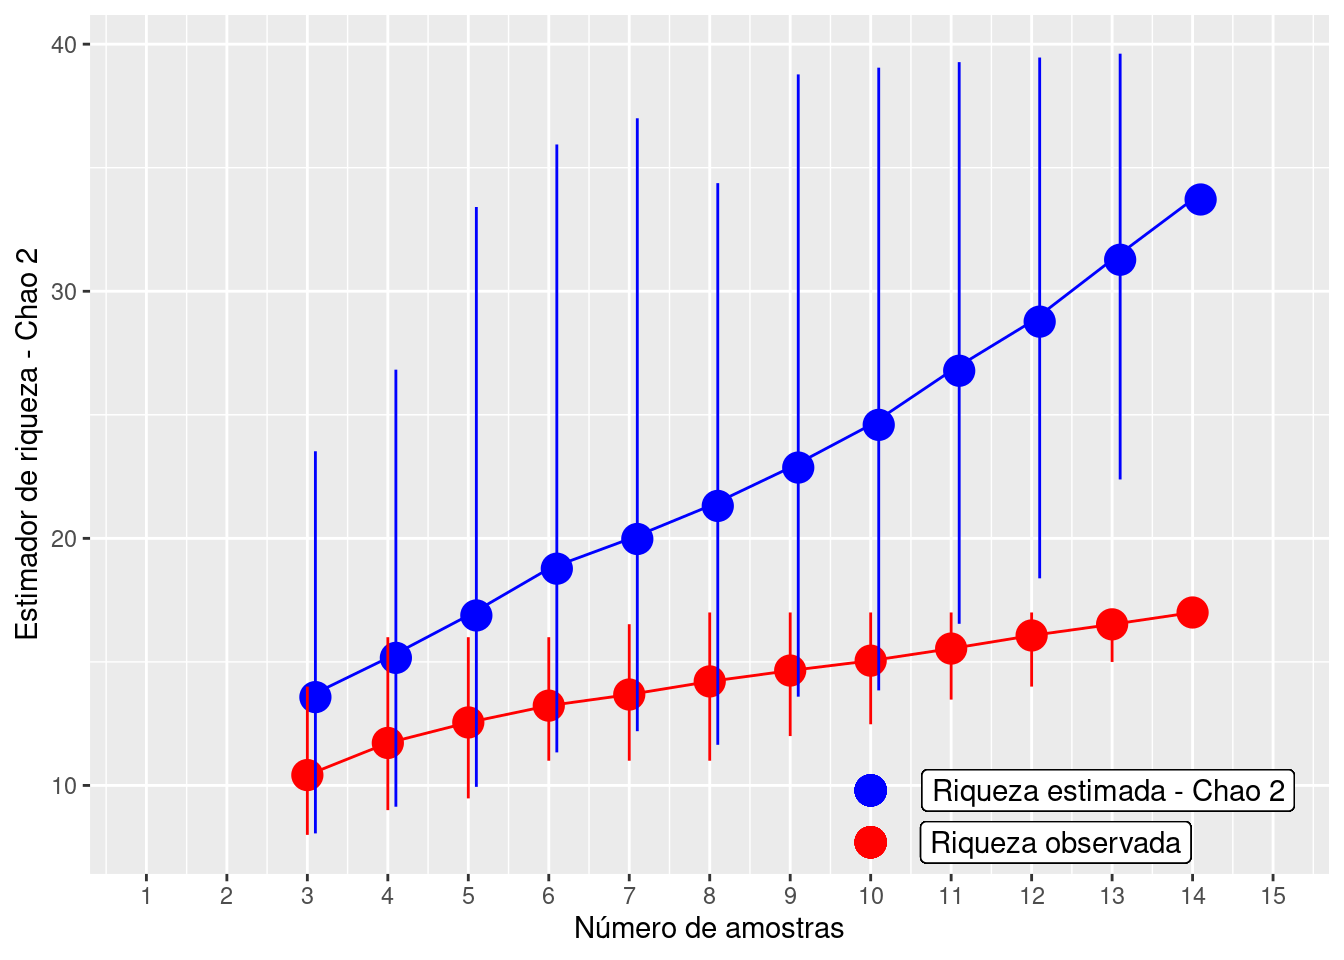
\includegraphics{livro_r_ecologia_files/figure-latex/unnamed-chunk-10-1.pdf}

\hypertarget{interpretauxe7uxe3o-dos-resultados-3}{%
\subsubsection{Interpretação dos resultados}\label{interpretauxe7uxe3o-dos-resultados-3}}

Com base no número de espécies raras (\emph{uniques} e \emph{duplicates}), Chao 2 estimou a possibilidade de encontrarmos mais dezesseis espécies caso o esforço amostral fosse maior e não mostrou tendência de estabilização da curva em uma assíntota.

\hypertarget{jackknife-1-burnham-overton-1978-1979}{%
\subsection{\texorpdfstring{\textbf{JACKKNIFE 1 (Burnham \& Overton 1978, 1979):}}{JACKKNIFE 1 (Burnham \& Overton 1978, 1979):}}\label{jackknife-1-burnham-overton-1978-1979}}

Este estimador baseia-se no número de espécies que ocorrem em somente uma amostra (Q1).

\begin{quote}
\[S_{jack1} = S_{obs} + Q1\left(\frac{m - 1}{m}\right)\]
\end{quote}

onde:

\begin{itemize}
\item
  Sobs = o número de espécies na comunidade,
\item
  Q1 = número de espécies observadas em uma amostragem (espécies \emph{uniques}),
\item
  \emph{m} = número de amostragens.
\end{itemize}

Palmer (1990) verificou que Jackknife 1 foi o estimador mais preciso e menos enviesado comparado a outros métodos de extrapolação.

~

\hypertarget{exemplo-pruxe1tico---jackknife-1}{%
\subsubsection{Exemplo prático - Jackknife 1}\label{exemplo-pruxe1tico---jackknife-1}}

\hypertarget{explicauxe7uxe3o-dos-dados-4}{%
\paragraph{Explicação dos dados}\label{explicauxe7uxe3o-dos-dados-4}}

Usaremos os mesmos dados de 17 espécies de anuros amostradas em 14 dias de coletas de campo em um habitat reprodutivo localizado na região noroeste do estado de São Paulo, Brasil.

\textbf{Pergunta:}

\begin{quote}
Quantas espécies a mais poderiam ser amostradas caso aumentasse o esforço amostral?
\end{quote}

\textbf{Predições}

\begin{quote}
\begin{itemize}
\tightlist
\item
  O número de espécies estimadas é similar ao número de espécies observada;
\item
  O número de espécies estimadas é maior do que o número de espécies observada.
\end{itemize}
\end{quote}

\textbf{Variáveis}

\begin{itemize}
\tightlist
\item
  Variáveis preditoras

  \begin{itemize}
  \tightlist
  \item
    matriz ou vetor com as abundâncias das espécies de anuros registradas em uma habitat reprodutivo
  \end{itemize}
\end{itemize}

\textbf{Checklist}

\begin{itemize}
\tightlist
\item
  Verificar se a sua matriz está com as espécies nas colunas e as amostragens nas linhas
\end{itemize}

\hypertarget{anuxe1lise-5}{%
\subsection{Análise}\label{anuxe1lise-5}}

Calculo do estimador de riqueza - Jackknife 1

\begin{Shaded}
\begin{Highlighting}[]
\KeywordTok{library}\NormalTok{(vegan)}
\NormalTok{dados_coleta <-}\StringTok{ }\NormalTok{poca_anuros}
\NormalTok{est_jack1 <-}\StringTok{ }\KeywordTok{poolaccum}\NormalTok{(dados_coleta, }\DataTypeTok{permutations =} \DecValTok{100}\NormalTok{)}
\KeywordTok{summary}\NormalTok{(est_jack1, }\DataTypeTok{display =} \StringTok{"jack1"}\NormalTok{)}
\end{Highlighting}
\end{Shaded}

\begin{verbatim}
## $jack1
##        N Jackknife 1      2.5%    97.5%  Std.Dev
##  [1,]  3    14.33000  8.491667 19.50833 2.862543
##  [2,]  4    15.24750  9.750000 20.64375 2.938661
##  [3,]  5    16.01800  9.695000 21.60000 3.065098
##  [4,]  6    17.03833 11.308333 22.35833 2.914307
##  [5,]  7    17.68286 12.264286 23.45000 2.926192
##  [6,]  8    18.50500 13.750000 23.58437 2.678591
##  [7,]  9    19.36778 14.777778 24.11111 2.598440
##  [8,] 10    19.81300 14.800000 24.20000 2.568364
##  [9,] 11    20.64000 16.727273 24.27273 2.210438
## [10,] 12    21.24333 17.185417 23.41667 1.985557
## [11,] 13    21.99462 18.692308 23.46154 1.346681
## [12,] 14    22.57143 22.571429 22.57143 0.000000
## 
## attr(,"class")
## [1] "summary.poolaccum"
\end{verbatim}

Visualizar os resultados com 95\% intervalo de confiança

\begin{Shaded}
\begin{Highlighting}[]
\KeywordTok{library}\NormalTok{(ggplot2)}
\CommentTok{# preparando os dados para fazer o gráfico}
\NormalTok{resultados_jack1 <-}\StringTok{ }\KeywordTok{summary}\NormalTok{(est_jack1, }\DataTypeTok{display =} \KeywordTok{c}\NormalTok{(}\StringTok{"S"}\NormalTok{, }\StringTok{"jack1"}\NormalTok{))}
\NormalTok{res_jack1 <-}\StringTok{ }\KeywordTok{cbind}\NormalTok{(resultados_jack1}\OperatorTok{$}\NormalTok{jack1[,}\DecValTok{1}\OperatorTok{:}\DecValTok{4}\NormalTok{], resultados_jack1}\OperatorTok{$}\NormalTok{S[,}\DecValTok{2}\OperatorTok{:}\DecValTok{4}\NormalTok{])}
\NormalTok{res_jack1 <-}\StringTok{ }\KeywordTok{as.data.frame}\NormalTok{(res_jack1)}
\KeywordTok{colnames}\NormalTok{(res_jack1) <-}\StringTok{ }\KeywordTok{c}\NormalTok{(}\StringTok{"Amostras"}\NormalTok{, }\StringTok{"JACK1"}\NormalTok{, }\StringTok{"JACK1_inferior"}\NormalTok{, }\StringTok{"JACK1_superior"}\NormalTok{, }\StringTok{"Riqueza"}\NormalTok{,}
                        \StringTok{"R_inferior"}\NormalTok{, }\StringTok{"R_superior"}\NormalTok{)}

\CommentTok{# comando para o gráfico}
\KeywordTok{ggplot}\NormalTok{(res_jack1, }\KeywordTok{aes}\NormalTok{(}\DataTypeTok{y =}\NormalTok{ Riqueza, }\DataTypeTok{x =}\NormalTok{ Amostras)) }\OperatorTok{+}
\StringTok{  }\KeywordTok{geom_point}\NormalTok{(}\KeywordTok{aes}\NormalTok{(}\DataTypeTok{y =}\NormalTok{ JACK1, }\DataTypeTok{x =}\NormalTok{ Amostras }\OperatorTok{+}\StringTok{ }\FloatTok{0.1}\NormalTok{), }\DataTypeTok{size =} \DecValTok{5}\NormalTok{, }\DataTypeTok{color =} \StringTok{"blue"}\NormalTok{, }\DataTypeTok{alpha =} \DecValTok{1}\NormalTok{) }\OperatorTok{+}
\StringTok{  }\KeywordTok{geom_point}\NormalTok{(}\KeywordTok{aes}\NormalTok{(}\DataTypeTok{y =}\NormalTok{ Riqueza, }\DataTypeTok{x =}\NormalTok{ Amostras), }\DataTypeTok{size =} \DecValTok{5}\NormalTok{, }\DataTypeTok{color =} \StringTok{"red"}\NormalTok{, }\DataTypeTok{alpha =} \DecValTok{1}\NormalTok{) }\OperatorTok{+}
\StringTok{  }\KeywordTok{geom_line}\NormalTok{ (}\KeywordTok{aes}\NormalTok{(}\DataTypeTok{y =}\NormalTok{ JACK1, }\DataTypeTok{x =}\NormalTok{ Amostras), }\DataTypeTok{color =} \StringTok{"blue"}\NormalTok{) }\OperatorTok{+}
\StringTok{  }\KeywordTok{geom_line}\NormalTok{ (}\KeywordTok{aes}\NormalTok{(}\DataTypeTok{y =}\NormalTok{ Riqueza, }\DataTypeTok{x =}\NormalTok{ Amostras), }\DataTypeTok{color =} \StringTok{"red"}\NormalTok{) }\OperatorTok{+}
\StringTok{  }\KeywordTok{geom_linerange}\NormalTok{(}\KeywordTok{aes}\NormalTok{(}\DataTypeTok{ymin =}\NormalTok{ JACK1_inferior, }\DataTypeTok{ymax =}\NormalTok{ JACK1_superior, }\DataTypeTok{x =}\NormalTok{ Amostras }\OperatorTok{+}\StringTok{ }\FloatTok{0.1}\NormalTok{),}
 \DataTypeTok{color =} \StringTok{"blue"}\NormalTok{) }\OperatorTok{+}
\StringTok{  }\KeywordTok{geom_linerange}\NormalTok{(}\KeywordTok{aes}\NormalTok{(}\DataTypeTok{ymin =}\NormalTok{ R_inferior, }\DataTypeTok{ymax =}\NormalTok{ R_superior, }\DataTypeTok{x =}\NormalTok{ Amostras), }\DataTypeTok{color =} \StringTok{"red"}\NormalTok{) }\OperatorTok{+}
\StringTok{  }\KeywordTok{ylab}\NormalTok{ (}\StringTok{"Estimador de riqueza - Jackknife 1"}\NormalTok{) }\OperatorTok{+}
\StringTok{  }\KeywordTok{xlab}\NormalTok{ (}\StringTok{"Número de amostras"}\NormalTok{) }\OperatorTok{+}
\StringTok{  }\KeywordTok{scale_x_continuous}\NormalTok{(}\DataTypeTok{limits =} \KeywordTok{c}\NormalTok{(}\DecValTok{1}\NormalTok{,}\DecValTok{15}\NormalTok{), }\DataTypeTok{breaks=}\KeywordTok{seq}\NormalTok{(}\DecValTok{1}\NormalTok{,}\DecValTok{15}\NormalTok{,}\DecValTok{1}\NormalTok{)) }\OperatorTok{+}
\StringTok{  }\KeywordTok{geom_point}\NormalTok{(}\DataTypeTok{y=} \FloatTok{9.9}\NormalTok{, }\DataTypeTok{x =} \DecValTok{9}\NormalTok{, }\DataTypeTok{size =} \DecValTok{5}\NormalTok{, }\DataTypeTok{color =} \StringTok{"blue"}\NormalTok{, }\DataTypeTok{alpha =} \DecValTok{1}\NormalTok{) }\OperatorTok{+}\StringTok{ }
\StringTok{  }\KeywordTok{geom_point}\NormalTok{(}\DataTypeTok{y=} \FloatTok{8.6}\NormalTok{, }\DataTypeTok{x =} \DecValTok{9}\NormalTok{, }\DataTypeTok{size =} \DecValTok{5}\NormalTok{, }\DataTypeTok{color =} \StringTok{"red"}\NormalTok{, }\DataTypeTok{alpha =} \DecValTok{1}\NormalTok{) }\OperatorTok{+}\StringTok{ }
\StringTok{  }\KeywordTok{geom_label}\NormalTok{( }\DataTypeTok{y =} \FloatTok{9.9}\NormalTok{, }\DataTypeTok{x =} \FloatTok{12.5}\NormalTok{, }\DataTypeTok{label =} \StringTok{"Riqueza estimada - Jackknife 1"}\NormalTok{) }\OperatorTok{+}
\StringTok{  }\KeywordTok{geom_label}\NormalTok{( }\DataTypeTok{y =} \FloatTok{8.6}\NormalTok{, }\DataTypeTok{x =} \FloatTok{11.5}\NormalTok{, }\DataTypeTok{label =} \StringTok{"Riqueza observada"}\NormalTok{)}
\end{Highlighting}
\end{Shaded}

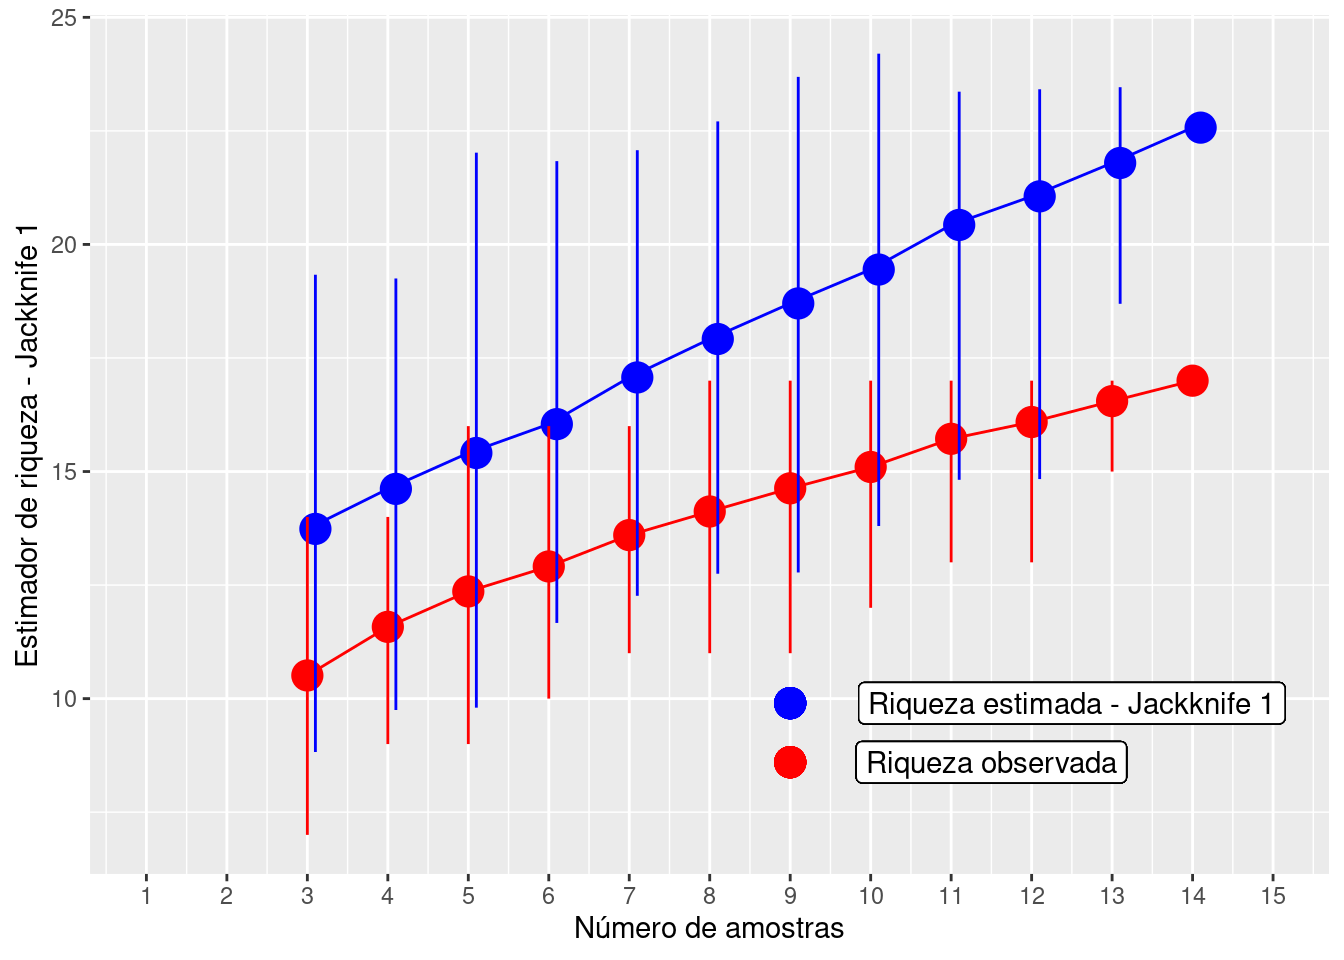
\includegraphics{livro_r_ecologia_files/figure-latex/unnamed-chunk-12-1.pdf}

\hypertarget{interpretauxe7uxe3o-dos-resultados-4}{%
\subsubsection{Interpretação dos resultados}\label{interpretauxe7uxe3o-dos-resultados-4}}

Com base no número de espécies raras, o estimador Jackknife 1 calculou a possibilidade de encontrarmos mais seis espécies caso o esforço amostral fosse maior e não mostrou tendência de estabilização da curva em uma assíntota.

\hypertarget{jackknife-2-burnham-overton-1978-1979-palmer-1991}{%
\subsection{\texorpdfstring{\textbf{JACKKNIFE 2 (Burnham \& Overton 1978, 1979, Palmer 1991):}}{JACKKNIFE 2 (Burnham \& Overton 1978, 1979, Palmer 1991):}}\label{jackknife-2-burnham-overton-1978-1979-palmer-1991}}

Este método basea-se no número de espécies que ocorrem em apenas uma amostra e no número de espécies que ocorrem em exatamente duas amostras.

\begin{quote}
\[S_{jack2} = S_{obs} + \left[\frac{Q_1(2m - 3)}{m}-\frac{Q_2(m - 2)^2}{m(m-1)}\right]\]
\end{quote}

onde:

\begin{itemize}
\item
  Sobs = o número de espécies na comunidade,
\item
  \emph{m} = número de amostragens,
\item
  Q1 = número de espécies observadas em uma amostragem (espécies \emph{uniques}),
\item
  Q2 = número de espécies observadas em duas amostragens (espécies \emph{duplicates}).
\end{itemize}

~

\hypertarget{exemplo-pruxe1tico---jackknife-2}{%
\subsubsection{Exemplo prático - Jackknife 2}\label{exemplo-pruxe1tico---jackknife-2}}

\hypertarget{explicauxe7uxe3o-dos-dados-5}{%
\paragraph{Explicação dos dados}\label{explicauxe7uxe3o-dos-dados-5}}

Usaremos os mesmos dados de 17 espécies de anuros amostradas em 14 dias de coletas de campo em um habitat reprodutivo localizado na região noroeste do estado de São Paulo, Brasil.

\textbf{Pergunta:}

\begin{quote}
Quantas espécies a mais poderiam ser amostradas caso aumentasse o esforço amostral?
\end{quote}

\textbf{Predições}

\begin{quote}
\begin{itemize}
\tightlist
\item
  O número de espécies estimadas é similar ao número de espécies observada;
\item
  O número de espécies estimadas é maior do que o número de espécies observada.
\end{itemize}
\end{quote}

\textbf{Variáveis}

\begin{itemize}
\tightlist
\item
  Variáveis preditoras

  \begin{itemize}
  \tightlist
  \item
    matriz ou vetor com as abundâncias das espécies de anuros registradas em uma habitat reprodutivo
  \end{itemize}
\end{itemize}

\textbf{Checklist}

\begin{itemize}
\tightlist
\item
  Verificar se a sua matriz está com as espécies nas colunas e as amostragens nas linhas
\end{itemize}

\hypertarget{anuxe1lise-6}{%
\subsection{Análise}\label{anuxe1lise-6}}

Calculo do estimador de riqueza - Jackknife 2

\begin{Shaded}
\begin{Highlighting}[]
\KeywordTok{library}\NormalTok{(vegan)}
\NormalTok{dados_coleta <-}\StringTok{ }\NormalTok{poca_anuros}
\NormalTok{est_jack2 <-}\StringTok{ }\KeywordTok{poolaccum}\NormalTok{(dados_coleta, }\DataTypeTok{permutations =} \DecValTok{100}\NormalTok{)}
\KeywordTok{summary}\NormalTok{(est_jack2, }\DataTypeTok{display =} \StringTok{"jack2"}\NormalTok{)}
\end{Highlighting}
\end{Shaded}

\begin{verbatim}
## $jack2
##        N Jackknife 2      2.5%    97.5%  Std.Dev
##  [1,]  3    14.90167  8.245833 22.85833 3.694955
##  [2,]  4    16.13250  8.233333 23.66667 4.175060
##  [3,]  5    16.90200  9.595000 24.66000 4.386607
##  [4,]  6    18.09033 12.137500 25.74500 3.812365
##  [5,]  7    18.67238 11.380952 27.00000 4.209857
##  [6,]  8    19.63446 11.339286 27.37500 4.294338
##  [7,]  9    20.59889 12.137847 27.83437 4.310667
##  [8,] 10    21.57467 13.285833 28.18889 4.112883
##  [9,] 11    22.84109 14.981818 28.35455 3.602369
## [10,] 12    23.96939 20.242424 28.49242 2.739930
## [11,] 13    25.47263 21.301282 27.76859 2.202224
## [12,] 14    26.92308 26.923077 26.92308 0.000000
## 
## attr(,"class")
## [1] "summary.poolaccum"
\end{verbatim}

Visualizar os resultados com intervalo de confiança de 95\%

\begin{Shaded}
\begin{Highlighting}[]
\KeywordTok{library}\NormalTok{(ggplot2)}
\CommentTok{# preparando os dados para fazer o gráfico}
\NormalTok{resultados_jack2 <-}\StringTok{ }\KeywordTok{summary}\NormalTok{(est_jack2, }\DataTypeTok{display =} \KeywordTok{c}\NormalTok{(}\StringTok{"S"}\NormalTok{, }\StringTok{"jack2"}\NormalTok{))}
\NormalTok{res_jack2 <-}\StringTok{ }\KeywordTok{cbind}\NormalTok{(resultados_jack2}\OperatorTok{$}\NormalTok{jack2[,}\DecValTok{1}\OperatorTok{:}\DecValTok{4}\NormalTok{], resultados_jack2}\OperatorTok{$}\NormalTok{S[,}\DecValTok{2}\OperatorTok{:}\DecValTok{4}\NormalTok{])}
\NormalTok{res_jack2 <-}\StringTok{ }\KeywordTok{as.data.frame}\NormalTok{(res_jack2)}
\KeywordTok{colnames}\NormalTok{(res_jack2) <-}\StringTok{ }\KeywordTok{c}\NormalTok{(}\StringTok{"Amostras"}\NormalTok{, }\StringTok{"JACK2"}\NormalTok{, }\StringTok{"JACK2_inferior"}\NormalTok{, }\StringTok{"JACK2_superior"}\NormalTok{, }\StringTok{"Riqueza"}\NormalTok{,}
                        \StringTok{"R_inferior"}\NormalTok{, }\StringTok{"R_superior"}\NormalTok{)}

\CommentTok{# comando para o gráfico}
\KeywordTok{ggplot}\NormalTok{(res_jack2, }\KeywordTok{aes}\NormalTok{(}\DataTypeTok{y =}\NormalTok{ Riqueza, }\DataTypeTok{x =}\NormalTok{ Amostras)) }\OperatorTok{+}
\StringTok{  }\KeywordTok{geom_point}\NormalTok{(}\KeywordTok{aes}\NormalTok{(}\DataTypeTok{y =}\NormalTok{ JACK2, }\DataTypeTok{x =}\NormalTok{ Amostras }\OperatorTok{+}\StringTok{ }\FloatTok{0.1}\NormalTok{), }\DataTypeTok{size =} \DecValTok{5}\NormalTok{, }\DataTypeTok{color =} \StringTok{"blue"}\NormalTok{, }\DataTypeTok{alpha =} \DecValTok{1}\NormalTok{) }\OperatorTok{+}
\StringTok{  }\KeywordTok{geom_point}\NormalTok{(}\KeywordTok{aes}\NormalTok{(}\DataTypeTok{y =}\NormalTok{ Riqueza, }\DataTypeTok{x =}\NormalTok{ Amostras), }\DataTypeTok{size =} \DecValTok{5}\NormalTok{, }\DataTypeTok{color =} \StringTok{"red"}\NormalTok{, }\DataTypeTok{alpha =} \DecValTok{1}\NormalTok{) }\OperatorTok{+}
\StringTok{  }\KeywordTok{geom_line}\NormalTok{ (}\KeywordTok{aes}\NormalTok{(}\DataTypeTok{y =}\NormalTok{ JACK2, }\DataTypeTok{x =}\NormalTok{ Amostras), }\DataTypeTok{color =} \StringTok{"blue"}\NormalTok{) }\OperatorTok{+}
\StringTok{  }\KeywordTok{geom_line}\NormalTok{ (}\KeywordTok{aes}\NormalTok{(}\DataTypeTok{y =}\NormalTok{ Riqueza, }\DataTypeTok{x =}\NormalTok{ Amostras), }\DataTypeTok{color =} \StringTok{"red"}\NormalTok{) }\OperatorTok{+}
\StringTok{  }\KeywordTok{geom_linerange}\NormalTok{(}\KeywordTok{aes}\NormalTok{(}\DataTypeTok{ymin =}\NormalTok{ JACK2_inferior, }\DataTypeTok{ymax =}\NormalTok{ JACK2_superior, }\DataTypeTok{x =}\NormalTok{ Amostras }\OperatorTok{+}\StringTok{ }\FloatTok{0.1}\NormalTok{),}
 \DataTypeTok{color =} \StringTok{"blue"}\NormalTok{) }\OperatorTok{+}
\StringTok{  }\KeywordTok{geom_linerange}\NormalTok{(}\KeywordTok{aes}\NormalTok{(}\DataTypeTok{ymin =}\NormalTok{ R_inferior, }\DataTypeTok{ymax =}\NormalTok{ R_superior, }\DataTypeTok{x =}\NormalTok{ Amostras), }\DataTypeTok{color =} \StringTok{"red"}\NormalTok{) }\OperatorTok{+}
\StringTok{  }\KeywordTok{ylab}\NormalTok{ (}\StringTok{"Estimador de riqueza - Jackknife 2"}\NormalTok{) }\OperatorTok{+}
\StringTok{  }\KeywordTok{xlab}\NormalTok{ (}\StringTok{"Número de amostras"}\NormalTok{) }\OperatorTok{+}
\StringTok{  }\KeywordTok{scale_x_continuous}\NormalTok{(}\DataTypeTok{limits =} \KeywordTok{c}\NormalTok{(}\DecValTok{1}\NormalTok{,}\DecValTok{15}\NormalTok{), }\DataTypeTok{breaks=}\KeywordTok{seq}\NormalTok{(}\DecValTok{1}\NormalTok{,}\DecValTok{15}\NormalTok{,}\DecValTok{1}\NormalTok{)) }\OperatorTok{+}
\StringTok{  }\KeywordTok{geom_point}\NormalTok{(}\DataTypeTok{y=} \FloatTok{9.9}\NormalTok{, }\DataTypeTok{x =} \DecValTok{9}\NormalTok{, }\DataTypeTok{size =} \DecValTok{5}\NormalTok{, }\DataTypeTok{color =} \StringTok{"blue"}\NormalTok{, }\DataTypeTok{alpha =} \DecValTok{1}\NormalTok{) }\OperatorTok{+}\StringTok{ }
\StringTok{  }\KeywordTok{geom_point}\NormalTok{(}\DataTypeTok{y=} \FloatTok{8.2}\NormalTok{, }\DataTypeTok{x =} \DecValTok{9}\NormalTok{, }\DataTypeTok{size =} \DecValTok{5}\NormalTok{, }\DataTypeTok{color =} \StringTok{"red"}\NormalTok{, }\DataTypeTok{alpha =} \DecValTok{1}\NormalTok{) }\OperatorTok{+}\StringTok{ }
\StringTok{  }\KeywordTok{geom_label}\NormalTok{( }\DataTypeTok{y =} \FloatTok{9.9}\NormalTok{, }\DataTypeTok{x =} \FloatTok{12.5}\NormalTok{, }\DataTypeTok{label =} \StringTok{"Riqueza estimada - Jackknife 2"}\NormalTok{) }\OperatorTok{+}
\StringTok{  }\KeywordTok{geom_label}\NormalTok{( }\DataTypeTok{y =} \FloatTok{8.2}\NormalTok{, }\DataTypeTok{x =} \FloatTok{11.5}\NormalTok{, }\DataTypeTok{label =} \StringTok{"Riqueza observada"}\NormalTok{)}
\end{Highlighting}
\end{Shaded}

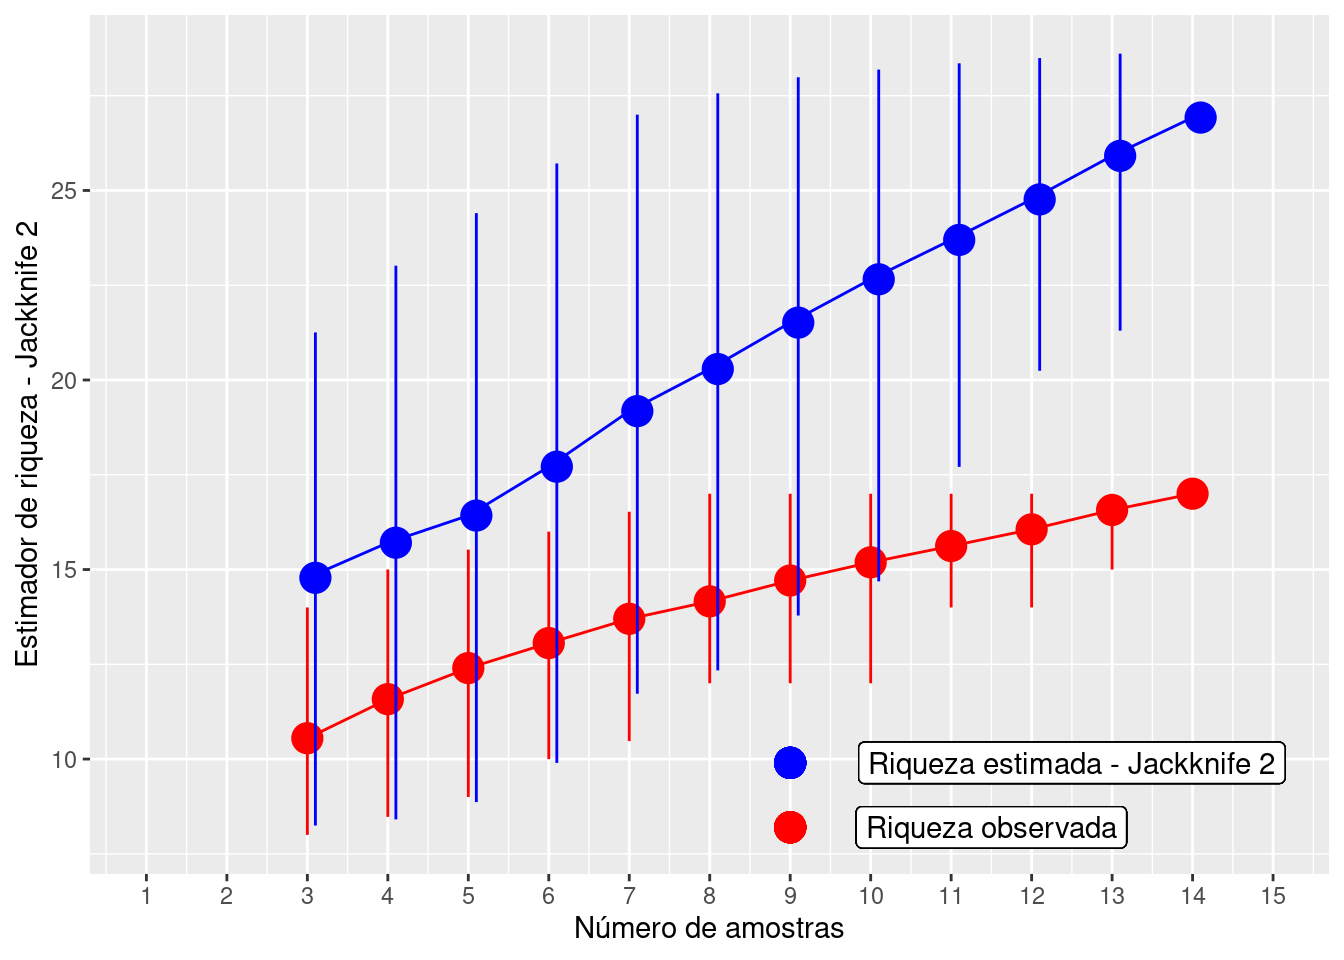
\includegraphics{livro_r_ecologia_files/figure-latex/unnamed-chunk-14-1.pdf}

\hypertarget{interpretauxe7uxe3o-dos-resultados-5}{%
\subsubsection{Interpretação dos resultados}\label{interpretauxe7uxe3o-dos-resultados-5}}

Com base no número de espécies raras, o estimador Jackknife 2 calculou a possibilidade de encontrarmos mais dez espécies caso o esforço amostral fosse maior e não mostrou tendência estabilização da curva em uma assíntota.

\hypertarget{bootstrap-smith-van-belle-1984}{%
\subsection{\texorpdfstring{\textbf{BOOTSTRAP (Smith \& van Belle 1984):}}{BOOTSTRAP (Smith \& van Belle 1984):}}\label{bootstrap-smith-van-belle-1984}}

Este método difere dos demais por utilizar dados de todas as espécies coletadas para estimar a riqueza total, não se restringindo às espécies raras. Ele requer somente dados de incidência. A estimativa pelo bootstrap é calculada somando-se a riqueza observada à soma do inverso da proporção de amostras em que cada espécie ocorre.

\begin{quote}
\[S_{boot} = S_{obs} + \sum_{k=1}^{S_{obs}}(1-P_k)^m\]
\end{quote}

onde:

\begin{itemize}
\item
  Sobs = o número de espécies na comunidade,
\item
  \emph{m} = número de amostragens,
\item
  Pk = proporção do número de amostras em que cada espécie foi registrada.
\end{itemize}

~

\hypertarget{exemplo-pruxe1tico---bootstrap}{%
\subsubsection{Exemplo prático - Bootstrap}\label{exemplo-pruxe1tico---bootstrap}}

\hypertarget{explicauxe7uxe3o-dos-dados-6}{%
\paragraph{Explicação dos dados}\label{explicauxe7uxe3o-dos-dados-6}}

Usaremos os mesmos dados de 17 espécies de anuros amostradas em 14 dias de coletas de campo em um habitat reprodutivo localizado na região noroeste do estado de São Paulo, Brasil.

\textbf{Pergunta:}

\begin{quote}
Quantas espécies a mais poderiam ser amostradas caso aumentasse o esforço amostral?
\end{quote}

\textbf{Predições}

\begin{quote}
\begin{itemize}
\tightlist
\item
  O número de espécies estimadas é similar ao número de espécies observada;
\item
  O número de espécies estimadas é maior do que o número de espécies observada.
\end{itemize}
\end{quote}

\textbf{Variáveis}

\begin{itemize}
\tightlist
\item
  Variáveis preditoras

  \begin{itemize}
  \tightlist
  \item
    matriz ou vetor com as abundâncias das espécies de anuros registradas em uma habitat reprodutivo
  \end{itemize}
\end{itemize}

\textbf{Checklist}

\begin{itemize}
\tightlist
\item
  Verificar se a sua matriz está com as espécies nas colunas e as amostragens nas linhas
\end{itemize}

\hypertarget{anuxe1lise-7}{%
\subsection{Análise}\label{anuxe1lise-7}}

Calculo do estimador de riqueza - Bootstrap

\begin{Shaded}
\begin{Highlighting}[]
\KeywordTok{library}\NormalTok{(vegan)}
\NormalTok{dados_coleta <-}\StringTok{ }\NormalTok{poca_anuros}
\NormalTok{est_boot <-}\StringTok{ }\KeywordTok{poolaccum}\NormalTok{(dados_coleta, }\DataTypeTok{permutations =} \DecValTok{100}\NormalTok{)}
\KeywordTok{summary}\NormalTok{(est_boot, }\DataTypeTok{display =} \StringTok{"boot"}\NormalTok{)}
\end{Highlighting}
\end{Shaded}

\begin{verbatim}
## $boot
##        N Bootstrap      2.5%    97.5%   Std.Dev
##  [1,]  3  12.18444  8.758333 16.44444 2.1474126
##  [2,]  4  13.30664  9.240039 17.57764 2.2451795
##  [3,]  5  14.07554  9.940792 18.48081 2.2635092
##  [4,]  6  14.64922 10.586985 18.43860 2.2483145
##  [5,]  7  15.32220 11.168044 19.82298 2.1465792
##  [6,]  8  15.99913 11.815949 19.79632 2.1988141
##  [7,]  9  16.69624 12.204194 19.80692 2.1563549
##  [8,] 10  17.18133 12.728991 19.80358 1.9529784
##  [9,] 11  17.72813 13.958390 19.59628 1.6428295
## [10,] 12  18.27063 15.374450 19.70990 1.3404657
## [11,] 13  18.80446 16.570376 19.47661 0.9517369
## [12,] 14  19.27832 19.278321 19.27832 0.0000000
## 
## attr(,"class")
## [1] "summary.poolaccum"
\end{verbatim}

Visualizar os resultados com intervalo de confiança de 95\%

\begin{Shaded}
\begin{Highlighting}[]
\KeywordTok{library}\NormalTok{(ggplot2)}
\CommentTok{# preparando os dados para fazer o gráfico}
\NormalTok{resultados_boot <-}\StringTok{ }\KeywordTok{summary}\NormalTok{(est_boot, }\DataTypeTok{display =} \KeywordTok{c}\NormalTok{(}\StringTok{"S"}\NormalTok{, }\StringTok{"boot"}\NormalTok{))}
\NormalTok{res_boot <-}\StringTok{ }\KeywordTok{cbind}\NormalTok{(resultados_boot}\OperatorTok{$}\NormalTok{boot[,}\DecValTok{1}\OperatorTok{:}\DecValTok{4}\NormalTok{], resultados_boot}\OperatorTok{$}\NormalTok{S[,}\DecValTok{2}\OperatorTok{:}\DecValTok{4}\NormalTok{])}
\NormalTok{res_boot <-}\StringTok{ }\KeywordTok{as.data.frame}\NormalTok{(res_boot)}
\KeywordTok{colnames}\NormalTok{(res_boot) <-}\StringTok{ }\KeywordTok{c}\NormalTok{(}\StringTok{"Amostras"}\NormalTok{, }\StringTok{"BOOT"}\NormalTok{, }\StringTok{"BOOT_inferior"}\NormalTok{, }\StringTok{"BOOT_superior"}\NormalTok{, }\StringTok{"Riqueza"}\NormalTok{,}
                        \StringTok{"R_inferior"}\NormalTok{, }\StringTok{"R_superior"}\NormalTok{)}

\CommentTok{# comando para o gráfico}
\KeywordTok{ggplot}\NormalTok{(res_boot, }\KeywordTok{aes}\NormalTok{(}\DataTypeTok{y =}\NormalTok{ Riqueza, }\DataTypeTok{x =}\NormalTok{ Amostras)) }\OperatorTok{+}
\StringTok{  }\KeywordTok{geom_point}\NormalTok{(}\KeywordTok{aes}\NormalTok{(}\DataTypeTok{y =}\NormalTok{ BOOT, }\DataTypeTok{x =}\NormalTok{ Amostras }\OperatorTok{+}\StringTok{ }\FloatTok{0.1}\NormalTok{), }\DataTypeTok{size =} \DecValTok{5}\NormalTok{, }\DataTypeTok{color =} \StringTok{"blue"}\NormalTok{, }\DataTypeTok{alpha =} \DecValTok{1}\NormalTok{) }\OperatorTok{+}
\StringTok{  }\KeywordTok{geom_point}\NormalTok{(}\KeywordTok{aes}\NormalTok{(}\DataTypeTok{y =}\NormalTok{ Riqueza, }\DataTypeTok{x =}\NormalTok{ Amostras), }\DataTypeTok{size =} \DecValTok{5}\NormalTok{, }\DataTypeTok{color =} \StringTok{"red"}\NormalTok{, }\DataTypeTok{alpha =} \DecValTok{1}\NormalTok{) }\OperatorTok{+}
\StringTok{  }\KeywordTok{geom_line}\NormalTok{ (}\KeywordTok{aes}\NormalTok{(}\DataTypeTok{y =}\NormalTok{ BOOT, }\DataTypeTok{x =}\NormalTok{ Amostras), }\DataTypeTok{color =} \StringTok{"blue"}\NormalTok{) }\OperatorTok{+}
\StringTok{  }\KeywordTok{geom_line}\NormalTok{ (}\KeywordTok{aes}\NormalTok{(}\DataTypeTok{y =}\NormalTok{ Riqueza, }\DataTypeTok{x =}\NormalTok{ Amostras), }\DataTypeTok{color =} \StringTok{"red"}\NormalTok{) }\OperatorTok{+}
\StringTok{  }\KeywordTok{geom_linerange}\NormalTok{(}\KeywordTok{aes}\NormalTok{(}\DataTypeTok{ymin =}\NormalTok{ BOOT_inferior, }\DataTypeTok{ymax =}\NormalTok{ BOOT_superior, }\DataTypeTok{x =}\NormalTok{ Amostras }\OperatorTok{+}\StringTok{ }\FloatTok{0.1}\NormalTok{),}
 \DataTypeTok{color =} \StringTok{"blue"}\NormalTok{) }\OperatorTok{+}
\StringTok{  }\KeywordTok{geom_linerange}\NormalTok{(}\KeywordTok{aes}\NormalTok{(}\DataTypeTok{ymin =}\NormalTok{ R_inferior, }\DataTypeTok{ymax =}\NormalTok{ R_superior, }\DataTypeTok{x =}\NormalTok{ Amostras), }\DataTypeTok{color =} \StringTok{"red"}\NormalTok{) }\OperatorTok{+}
\StringTok{  }\KeywordTok{ylab}\NormalTok{ (}\StringTok{"Estimador de riqueza - Bootstrap"}\NormalTok{) }\OperatorTok{+}
\StringTok{  }\KeywordTok{xlab}\NormalTok{ (}\StringTok{"Número de amostras"}\NormalTok{) }\OperatorTok{+}
\StringTok{  }\KeywordTok{scale_x_continuous}\NormalTok{(}\DataTypeTok{limits =} \KeywordTok{c}\NormalTok{(}\DecValTok{1}\NormalTok{,}\DecValTok{15}\NormalTok{), }\DataTypeTok{breaks=}\KeywordTok{seq}\NormalTok{(}\DecValTok{1}\NormalTok{,}\DecValTok{15}\NormalTok{,}\DecValTok{1}\NormalTok{)) }\OperatorTok{+}
\StringTok{  }\KeywordTok{geom_point}\NormalTok{(}\DataTypeTok{y=} \FloatTok{10.4}\NormalTok{, }\DataTypeTok{x =} \FloatTok{9.5}\NormalTok{, }\DataTypeTok{size =} \DecValTok{5}\NormalTok{, }\DataTypeTok{color =} \StringTok{"blue"}\NormalTok{, }\DataTypeTok{alpha =} \DecValTok{1}\NormalTok{) }\OperatorTok{+}\StringTok{ }
\StringTok{  }\KeywordTok{geom_point}\NormalTok{(}\DataTypeTok{y=} \FloatTok{9.3}\NormalTok{, }\DataTypeTok{x =} \FloatTok{9.5}\NormalTok{, }\DataTypeTok{size =} \DecValTok{5}\NormalTok{, }\DataTypeTok{color =} \StringTok{"red"}\NormalTok{, }\DataTypeTok{alpha =} \DecValTok{1}\NormalTok{) }\OperatorTok{+}\StringTok{ }
\StringTok{  }\KeywordTok{geom_label}\NormalTok{( }\DataTypeTok{y =} \FloatTok{10.4}\NormalTok{, }\DataTypeTok{x =} \FloatTok{12.3}\NormalTok{, }\DataTypeTok{label =} \StringTok{"Riqueza estimada - Bootstrap"}\NormalTok{) }\OperatorTok{+}
\StringTok{  }\KeywordTok{geom_label}\NormalTok{( }\DataTypeTok{y =} \FloatTok{9.3}\NormalTok{, }\DataTypeTok{x =} \FloatTok{11.5}\NormalTok{, }\DataTypeTok{label =} \StringTok{"Riqueza observada"}\NormalTok{)}
\end{Highlighting}
\end{Shaded}

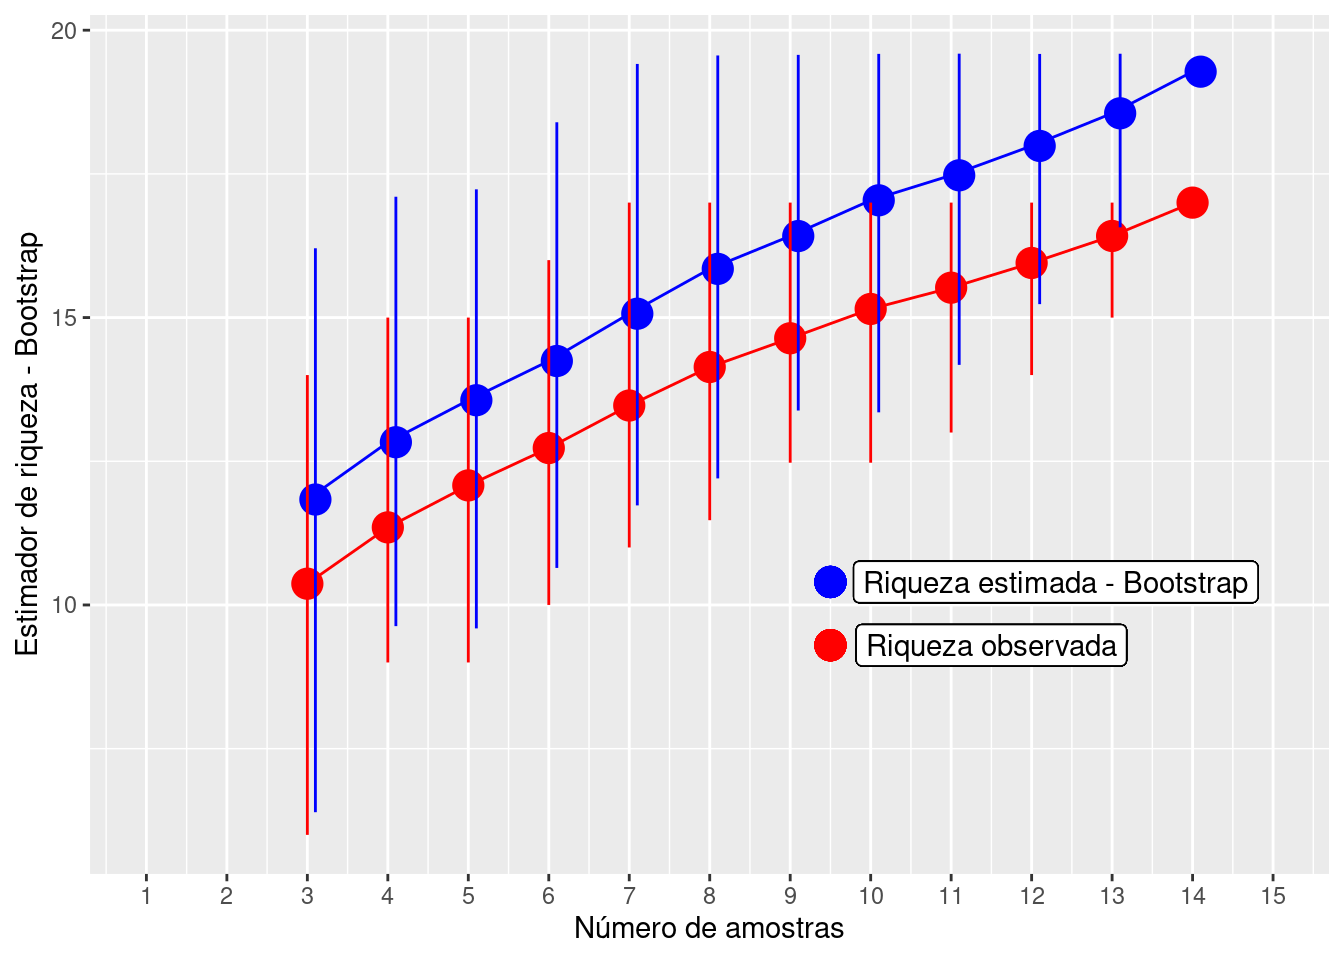
\includegraphics{livro_r_ecologia_files/figure-latex/unnamed-chunk-16-1.pdf}

\hypertarget{interpretauxe7uxe3o-dos-resultados-6}{%
\subsubsection{Interpretação dos resultados}\label{interpretauxe7uxe3o-dos-resultados-6}}

Com base na frequencia de ocorrência das espécies, o estimador bootstrap calculou a possibilidade de encontrarmos mais duas espécies caso o esforço amostral fosse maior e não mostrou tendência de estabilização da curva em uma assíntota.

\hypertarget{interpolauxe7uxe3o-e-extrapolauxe7uxe3o-baseadas-em-rarefauxe7uxe3o-usando-amostragens-de-inciduxeancia-ou-abunduxe2ncia-chao-jost-2012-colwell-et-al.-2012}{%
\subsection{\texorpdfstring{\textbf{Interpolação e Extrapolação baseadas em rarefação usando amostragens de incidência ou abundância (Chao \& Jost 2012, Colwell et al.~2012):}}{Interpolação e Extrapolação baseadas em rarefação usando amostragens de incidência ou abundância (Chao \& Jost 2012, Colwell et al.~2012):}}\label{interpolauxe7uxe3o-e-extrapolauxe7uxe3o-baseadas-em-rarefauxe7uxe3o-usando-amostragens-de-inciduxeancia-ou-abunduxe2ncia-chao-jost-2012-colwell-et-al.-2012}}

Este método utiliza teoria de amostragem (e.g.~modelos multinomial, Poisson e Bernoulli) para conectar rarefação (interpolação) e predição (extrapolação) com base no tamanho da amostra. Contudo, é importante enfatizar que a extrapolação torna-se altamente incerta quando extendida para o dobro do tamanho da amostragem. Este método utiliza uma abordagem com bootstrap para calcular o intervalo de confiança de 95\%.

\hypertarget{exemplo-pruxe1tico}{%
\subsubsection{Exemplo prático}\label{exemplo-pruxe1tico}}

\hypertarget{explicauxe7uxe3o-dos-dados-7}{%
\paragraph{Explicação dos dados}\label{explicauxe7uxe3o-dos-dados-7}}

Usaremos os mesmos dados de 17 espécies de anuros amostradas em 14 dias de coletas de campo em um habitat reprodutivo localizado na região noroeste do estado de São Paulo, Brasil.

\textbf{Pergunta:}

\begin{quote}
Quantas espécies a mais poderiam ser amostradas caso aumentasse o esforço amostral?
\end{quote}

\textbf{Predições}

\begin{quote}
\begin{itemize}
\tightlist
\item
  O número de espécies estimadas é similar ao número de espécies observada;
\item
  O número de espécies estimadas é maior do que o número de espécies observada.
\end{itemize}
\end{quote}

\textbf{Variáveis}

\begin{itemize}
\tightlist
\item
  Variáveis preditoras

  \begin{itemize}
  \tightlist
  \item
    matriz ou vetor com as abundâncias das espécies de anuros registradas em uma habitat reprodutivo
  \end{itemize}
\end{itemize}

\textbf{Checklist}

\begin{itemize}
\tightlist
\item
  Verificar se a sua matriz está com as espécies nas colunas e as amostragens nas linhas.
\end{itemize}

\hypertarget{anuxe1lise-8}{%
\subsection{Análise}\label{anuxe1lise-8}}

Calculo da extrapolação da riqueza com base no número de indivíduos

\begin{Shaded}
\begin{Highlighting}[]
\KeywordTok{library}\NormalTok{(iNEXT)}
\NormalTok{dados_coleta <-}\StringTok{ }\NormalTok{poca_anuros}

\CommentTok{# preparando os dados para análises considerando a abundância}
\NormalTok{dados_inext_abu <-}\StringTok{ }\KeywordTok{colSums}\NormalTok{(dados_coleta) }

\NormalTok{resultados_abundancia <-}\StringTok{ }\KeywordTok{iNEXT}\NormalTok{(dados_inext_abu, }\DataTypeTok{q =} \DecValTok{0}\NormalTok{, }\DataTypeTok{datatype =} \StringTok{"abundance"}\NormalTok{, }
            \DataTypeTok{endpoint =} \DecValTok{600}\NormalTok{)}

\CommentTok{# Visualizar os dados no gráfico}
\KeywordTok{ggiNEXT}\NormalTok{(resultados_abundancia, }\DataTypeTok{type =} \DecValTok{1}\NormalTok{)}
\end{Highlighting}
\end{Shaded}

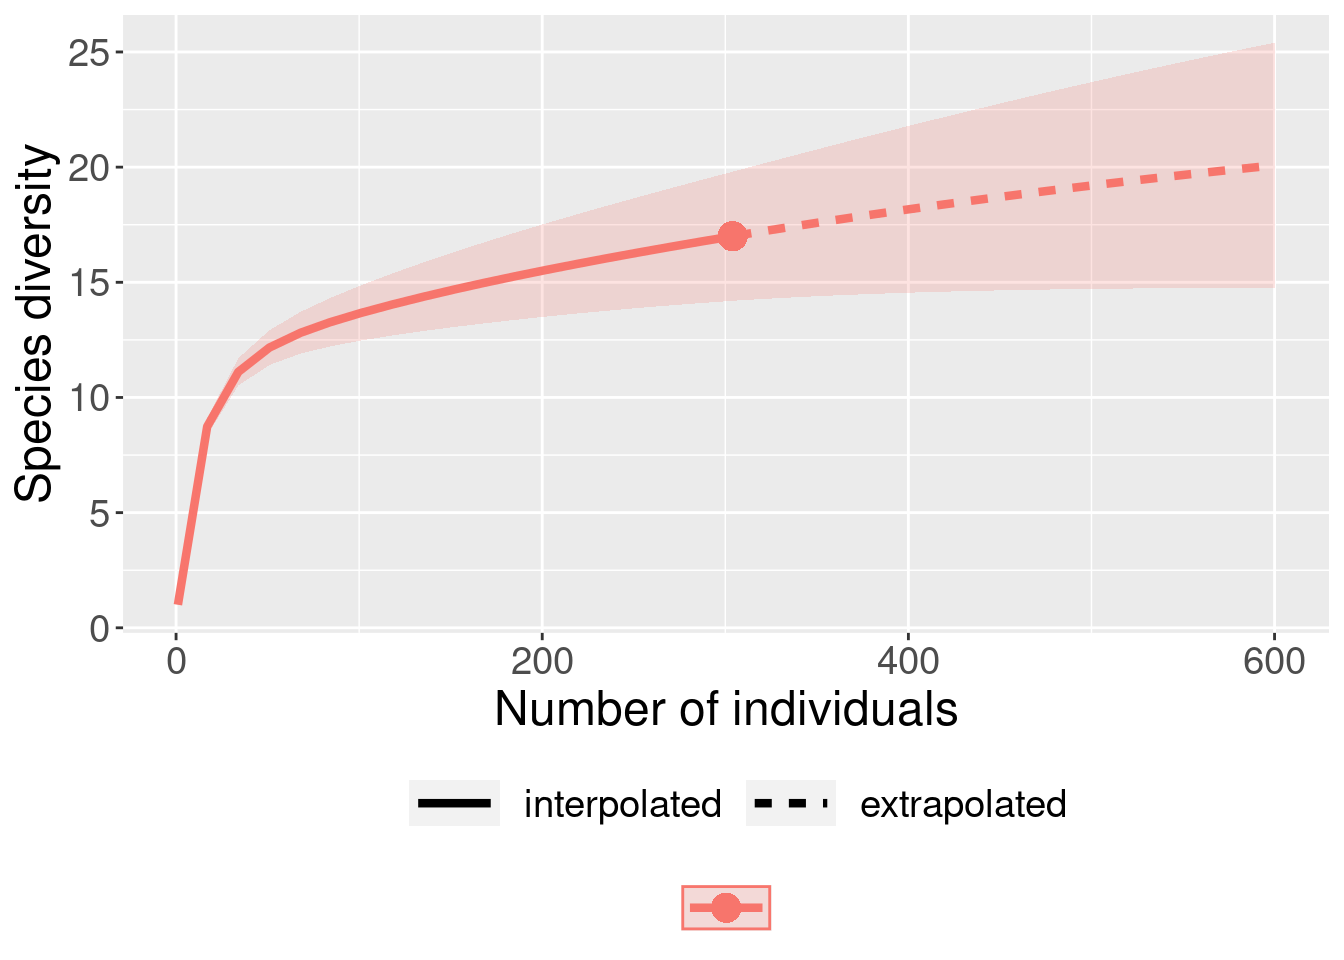
\includegraphics{livro_r_ecologia_files/figure-latex/unnamed-chunk-17-1.pdf}

\hypertarget{interpretauxe7uxe3o-dos-resultados-7}{%
\subsubsection{Interpretação dos resultados}\label{interpretauxe7uxe3o-dos-resultados-7}}

Veja que o ponto no final da linha contínua representa as 17 espécies de anuros (eixo Y) observadas entre os 304 individuos (eixo X). A extrapolação máxima (600 indivíduos no nosso exemplo), estima um aumento de até oito espécies (intervalo de confiança) caso amostrássemos mais 300 indivíduos.

Calculo da extrapolação da riqueza com base no número de amostras

\begin{Shaded}
\begin{Highlighting}[]
\KeywordTok{library}\NormalTok{(iNEXT)}
\NormalTok{dados_coleta <-}\StringTok{ }\NormalTok{poca_anuros}

\CommentTok{# preparando os dados para análises considerando a incidência}
\NormalTok{dados_inext <-}\StringTok{ }\KeywordTok{as.incfreq}\NormalTok{(}\KeywordTok{t}\NormalTok{(dados_coleta)) }\CommentTok{# preciso transpor o dataframe}
\end{Highlighting}
\end{Shaded}

\begin{verbatim}
## Warning in as.incfreq(t(dados_coleta)): Invalid data type, the element of
## species by sites presence-absence matrix should be 0 or 1. Set nonzero elements
## as 1.
\end{verbatim}

\begin{Shaded}
\begin{Highlighting}[]
\NormalTok{resultados_incidencia <-}\StringTok{ }\KeywordTok{iNEXT}\NormalTok{(dados_inext, }\DataTypeTok{q =} \DecValTok{0}\NormalTok{, }\DataTypeTok{datatype =} \StringTok{"incidence_freq"}\NormalTok{, }
            \DataTypeTok{endpoint =} \DecValTok{30}\NormalTok{)}

\CommentTok{# Visualizar os dados no gráfico}
\KeywordTok{ggiNEXT}\NormalTok{(resultados_incidencia, }\DataTypeTok{type =} \DecValTok{1}\NormalTok{)}
\end{Highlighting}
\end{Shaded}

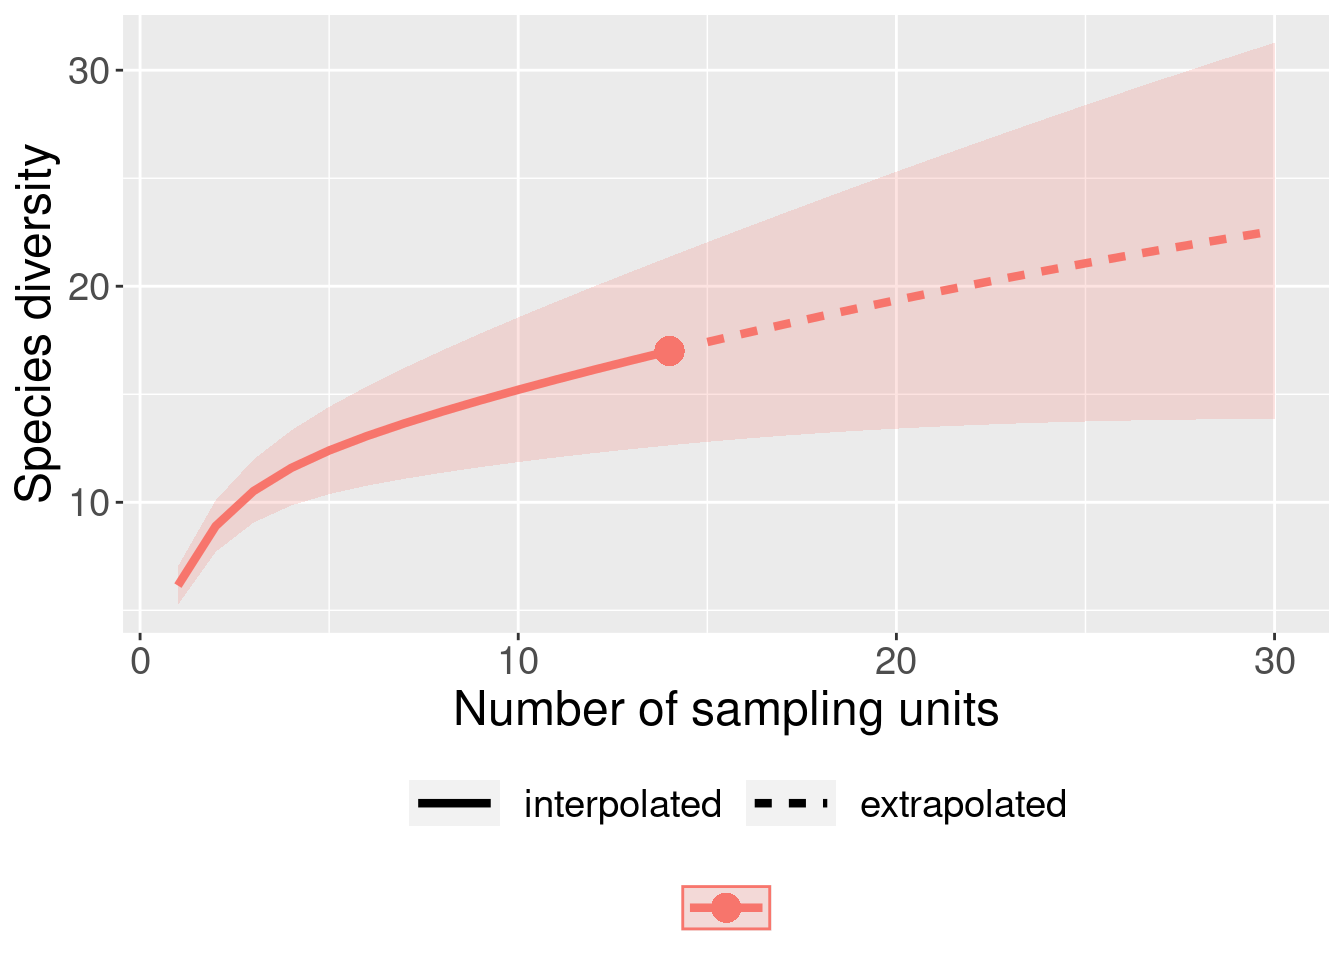
\includegraphics{livro_r_ecologia_files/figure-latex/unnamed-chunk-18-1.pdf}

\hypertarget{interpretauxe7uxe3o-dos-resultados-8}{%
\subsubsection{Interpretação dos resultados}\label{interpretauxe7uxe3o-dos-resultados-8}}

Veja que o ponto no final da linha contínua representa as 17 espécies de anuros (eixo Y) observadas nos 14 dias de coleta (eixo X - amostras). A extrapolação máxima (30 dias de coleta no nosso exemplo), estima um aumento de até 13 espécies (intervalo de confiança) caso amostrássemos mais 16 dias.

~

\hypertarget{para-se-aprofundar-1}{%
\subsection{\texorpdfstring{\textbf{Para se aprofundar}}{Para se aprofundar}}\label{para-se-aprofundar-1}}

\begin{itemize}
\item
  Recomendamos aos interessados que olhem a página do \href{http://viceroy.eeb.uconn.edu/estimates}{EstimateS software} e baixem o manual do usuário que contém informações detalhadas sobre os índices de rarefação e estimadores de riqueza.Este site foi criado e é mantido pelo Dr.~Robert K. Colwell, um dos maiores especialistas do mundo em estimativas da biodiversidade
\item
  Recomendamos também o livro Magurran \& McGill (2010) - Biological Diversity Frontiers in Measurement and Assessment.
\end{itemize}

\hypertarget{diversidade-filogenuxe9tica}{%
\chapter{Diversidade filogenética}\label{diversidade-filogenuxe9tica}}

Lorem ipsum dolor sit amet, consectetur adipiscing elit. Proin in nisi egestas, volutpat lectus non, interdum nunc. Lorem ipsum dolor sit amet, consectetur adipiscing elit. Ut nulla quam, fermentum consequat maximus tristique, ultricies eget nunc. Donec efficitur tristique est hendrerit eleifend. Mauris elementum arcu vitae ultrices congue. Proin accumsan sollicitudin augue et iaculis. Quisque id tempor elit. Interdum et malesuada fames ac ante ipsum primis in faucibus. Duis iaculis purus nisi, non luctus metus vulputate quis. Maecenas felis urna, tristique eu maximus non, placerat aliquet felis. Ut elit enim, consequat in metus facilisis, fringilla dignissim neque. Nunc vehicula nulla et euismod interdum. Donec quis sapien non mi aliquet laoreet. Sed fermentum diam eu tempor hendrerit. Sed varius orci sit amet massa pellentesque, commodo commodo velit auctor. Integer finibus erat vitae sapien mattis, et auctor augue tincidunt.

\hypertarget{sub-seuxe7uxe3o-1-2}{%
\section{Sub-seção 1}\label{sub-seuxe7uxe3o-1-2}}

Duis scelerisque porta massa id lacinia. Quisque sodales malesuada neque, at posuere justo. Sed nec diam vel sapien feugiat efficitur lobortis a massa. Vestibulum in finibus urna, in facilisis quam. Sed purus libero, lacinia id arcu in, volutpat tempor elit. Donec luctus tellus quis arcu porttitor aliquet. Duis pellentesque felis non dolor ullamcorper pharetra. Proin sit amet justo id metus tempus faucibus eget a dolor. Cras elementum massa et justo tempor placerat. Etiam ac metus interdum, efficitur magna sed, mattis velit.

\hypertarget{sub-seuxe7uxe3o-2-2}{%
\section{Sub-seção 2}\label{sub-seuxe7uxe3o-2-2}}

Duis nec nisi sapien. Aenean a metus faucibus, malesuada ante et, semper magna. Sed vel fermentum mauris. Duis consectetur eget risus condimentum tempus. Cras tincidunt dui sed rutrum mollis. Sed tincidunt condimentum odio at luctus. Quisque sed augue urna. Aenean vel turpis dignissim, finibus elit commodo, sagittis massa. Sed lacinia leo massa, a varius sapien dictum in. Sed at pellentesque velit. Quisque pretium est a nisi fringilla, at bibendum enim sagittis. Phasellus a facilisis orci. Mauris auctor dolor a nunc cursus, in mattis lorem euismod. Donec sed convallis felis.

\hypertarget{sub-seuxe7uxe3o-3-2}{%
\section{Sub-seção 3}\label{sub-seuxe7uxe3o-3-2}}

Nam tortor lacus, volutpat ac aliquam tincidunt, posuere eu dui. Donec auctor ante convallis diam laoreet, eget luctus lorem iaculis. Proin feugiat ipsum nec velit commodo bibendum. Phasellus aliquet metus vehicula convallis aliquam. Quisque pretium ut augue non mollis. Nulla ut pulvinar nisl, at blandit sem. Nam vitae pellentesque risus. Fusce rhoncus eros eget velit volutpat rhoncus. Nam tempor varius fringilla. Aliquam venenatis interdum lorem at pellentesque. Nam a risus vitae dolor maximus ullamcorper nec et diam. Nunc condimentum arcu eu lacinia pellentesque. Etiam at nulla felis.

\hypertarget{diversidade-funcional}{%
\chapter{Diversidade funcional}\label{diversidade-funcional}}

Lorem ipsum dolor sit amet, consectetur adipiscing elit. Proin in nisi egestas, volutpat lectus non, interdum nunc. Lorem ipsum dolor sit amet, consectetur adipiscing elit. Ut nulla quam, fermentum consequat maximus tristique, ultricies eget nunc. Donec efficitur tristique est hendrerit eleifend. Mauris elementum arcu vitae ultrices congue. Proin accumsan sollicitudin augue et iaculis. Quisque id tempor elit. Interdum et malesuada fames ac ante ipsum primis in faucibus. Duis iaculis purus nisi, non luctus metus vulputate quis. Maecenas felis urna, tristique eu maximus non, placerat aliquet felis. Ut elit enim, consequat in metus facilisis, fringilla dignissim neque. Nunc vehicula nulla et euismod interdum. Donec quis sapien non mi aliquet laoreet. Sed fermentum diam eu tempor hendrerit. Sed varius orci sit amet massa pellentesque, commodo commodo velit auctor. Integer finibus erat vitae sapien mattis, et auctor augue tincidunt.

\hypertarget{sub-seuxe7uxe3o-1-3}{%
\section{Sub-seção 1}\label{sub-seuxe7uxe3o-1-3}}

Duis scelerisque porta massa id lacinia. Quisque sodales malesuada neque, at posuere justo. Sed nec diam vel sapien feugiat efficitur lobortis a massa. Vestibulum in finibus urna, in facilisis quam. Sed purus libero, lacinia id arcu in, volutpat tempor elit. Donec luctus tellus quis arcu porttitor aliquet. Duis pellentesque felis non dolor ullamcorper pharetra. Proin sit amet justo id metus tempus faucibus eget a dolor. Cras elementum massa et justo tempor placerat. Etiam ac metus interdum, efficitur magna sed, mattis velit.

\hypertarget{sub-seuxe7uxe3o-2-3}{%
\section{Sub-seção 2}\label{sub-seuxe7uxe3o-2-3}}

Duis nec nisi sapien. Aenean a metus faucibus, malesuada ante et, semper magna. Sed vel fermentum mauris. Duis consectetur eget risus condimentum tempus. Cras tincidunt dui sed rutrum mollis. Sed tincidunt condimentum odio at luctus. Quisque sed augue urna. Aenean vel turpis dignissim, finibus elit commodo, sagittis massa. Sed lacinia leo massa, a varius sapien dictum in. Sed at pellentesque velit. Quisque pretium est a nisi fringilla, at bibendum enim sagittis. Phasellus a facilisis orci. Mauris auctor dolor a nunc cursus, in mattis lorem euismod. Donec sed convallis felis.

\hypertarget{sub-seuxe7uxe3o-3-3}{%
\section{Sub-seção 3}\label{sub-seuxe7uxe3o-3-3}}

Nam tortor lacus, volutpat ac aliquam tincidunt, posuere eu dui. Donec auctor ante convallis diam laoreet, eget luctus lorem iaculis. Proin feugiat ipsum nec velit commodo bibendum. Phasellus aliquet metus vehicula convallis aliquam. Quisque pretium ut augue non mollis. Nulla ut pulvinar nisl, at blandit sem. Nam vitae pellentesque risus. Fusce rhoncus eros eget velit volutpat rhoncus. Nam tempor varius fringilla. Aliquam venenatis interdum lorem at pellentesque. Nam a risus vitae dolor maximus ullamcorper nec et diam. Nunc condimentum arcu eu lacinia pellentesque. Etiam at nulla felis.

\hypertarget{visualizauxe7uxe3o-de-dados-no-espauxe7o}{%
\chapter{Visualização de dados no espaço}\label{visualizauxe7uxe3o-de-dados-no-espauxe7o}}

Lorem ipsum dolor sit amet, consectetur adipiscing elit. Proin in nisi egestas, volutpat lectus non, interdum nunc. Lorem ipsum dolor sit amet, consectetur adipiscing elit. Ut nulla quam, fermentum consequat maximus tristique, ultricies eget nunc. Donec efficitur tristique est hendrerit eleifend. Mauris elementum arcu vitae ultrices congue. Proin accumsan sollicitudin augue et iaculis. Quisque id tempor elit. Interdum et malesuada fames ac ante ipsum primis in faucibus. Duis iaculis purus nisi, non luctus metus vulputate quis. Maecenas felis urna, tristique eu maximus non, placerat aliquet felis. Ut elit enim, consequat in metus facilisis, fringilla dignissim neque. Nunc vehicula nulla et euismod interdum. Donec quis sapien non mi aliquet laoreet. Sed fermentum diam eu tempor hendrerit. Sed varius orci sit amet massa pellentesque, commodo commodo velit auctor. Integer finibus erat vitae sapien mattis, et auctor augue tincidunt.

\hypertarget{sub-seuxe7uxe3o-1-4}{%
\section{Sub-seção 1}\label{sub-seuxe7uxe3o-1-4}}

Duis scelerisque porta massa id lacinia. Quisque sodales malesuada neque, at posuere justo. Sed nec diam vel sapien feugiat efficitur lobortis a massa. Vestibulum in finibus urna, in facilisis quam. Sed purus libero, lacinia id arcu in, volutpat tempor elit. Donec luctus tellus quis arcu porttitor aliquet. Duis pellentesque felis non dolor ullamcorper pharetra. Proin sit amet justo id metus tempus faucibus eget a dolor. Cras elementum massa et justo tempor placerat. Etiam ac metus interdum, efficitur magna sed, mattis velit.

\hypertarget{sub-seuxe7uxe3o-2-4}{%
\section{Sub-seção 2}\label{sub-seuxe7uxe3o-2-4}}

Duis nec nisi sapien. Aenean a metus faucibus, malesuada ante et, semper magna. Sed vel fermentum mauris. Duis consectetur eget risus condimentum tempus. Cras tincidunt dui sed rutrum mollis. Sed tincidunt condimentum odio at luctus. Quisque sed augue urna. Aenean vel turpis dignissim, finibus elit commodo, sagittis massa. Sed lacinia leo massa, a varius sapien dictum in. Sed at pellentesque velit. Quisque pretium est a nisi fringilla, at bibendum enim sagittis. Phasellus a facilisis orci. Mauris auctor dolor a nunc cursus, in mattis lorem euismod. Donec sed convallis felis.

\hypertarget{sub-seuxe7uxe3o-3-4}{%
\section{Sub-seção 3}\label{sub-seuxe7uxe3o-3-4}}

Nam tortor lacus, volutpat ac aliquam tincidunt, posuere eu dui. Donec auctor ante convallis diam laoreet, eget luctus lorem iaculis. Proin feugiat ipsum nec velit commodo bibendum. Phasellus aliquet metus vehicula convallis aliquam. Quisque pretium ut augue non mollis. Nulla ut pulvinar nisl, at blandit sem. Nam vitae pellentesque risus. Fusce rhoncus eros eget velit volutpat rhoncus. Nam tempor varius fringilla. Aliquam venenatis interdum lorem at pellentesque. Nam a risus vitae dolor maximus ullamcorper nec et diam. Nunc condimentum arcu eu lacinia pellentesque. Etiam at nulla felis.

\hypertarget{reprodutibilidade-em-pesquisa-e-gerenciamento-de-dados}{%
\chapter{Reprodutibilidade em pesquisa e gerenciamento de dados}\label{reprodutibilidade-em-pesquisa-e-gerenciamento-de-dados}}

Lorem ipsum dolor sit amet, consectetur adipiscing elit. Proin in nisi egestas, volutpat lectus non, interdum nunc. Lorem ipsum dolor sit amet, consectetur adipiscing elit. Ut nulla quam, fermentum consequat maximus tristique, ultricies eget nunc. Donec efficitur tristique est hendrerit eleifend. Mauris elementum arcu vitae ultrices congue. Proin accumsan sollicitudin augue et iaculis. Quisque id tempor elit. Interdum et malesuada fames ac ante ipsum primis in faucibus. Duis iaculis purus nisi, non luctus metus vulputate quis. Maecenas felis urna, tristique eu maximus non, placerat aliquet felis. Ut elit enim, consequat in metus facilisis, fringilla dignissim neque. Nunc vehicula nulla et euismod interdum. Donec quis sapien non mi aliquet laoreet. Sed fermentum diam eu tempor hendrerit. Sed varius orci sit amet massa pellentesque, commodo commodo velit auctor. Integer finibus erat vitae sapien mattis, et auctor augue tincidunt.

\hypertarget{sub-seuxe7uxe3o-1-5}{%
\section{Sub-seção 1}\label{sub-seuxe7uxe3o-1-5}}

Duis scelerisque porta massa id lacinia. Quisque sodales malesuada neque, at posuere justo. Sed nec diam vel sapien feugiat efficitur lobortis a massa. Vestibulum in finibus urna, in facilisis quam. Sed purus libero, lacinia id arcu in, volutpat tempor elit. Donec luctus tellus quis arcu porttitor aliquet. Duis pellentesque felis non dolor ullamcorper pharetra. Proin sit amet justo id metus tempus faucibus eget a dolor. Cras elementum massa et justo tempor placerat. Etiam ac metus interdum, efficitur magna sed, mattis velit.

\hypertarget{sub-seuxe7uxe3o-2-5}{%
\section{Sub-seção 2}\label{sub-seuxe7uxe3o-2-5}}

Duis nec nisi sapien. Aenean a metus faucibus, malesuada ante et, semper magna. Sed vel fermentum mauris. Duis consectetur eget risus condimentum tempus. Cras tincidunt dui sed rutrum mollis. Sed tincidunt condimentum odio at luctus. Quisque sed augue urna. Aenean vel turpis dignissim, finibus elit commodo, sagittis massa. Sed lacinia leo massa, a varius sapien dictum in. Sed at pellentesque velit. Quisque pretium est a nisi fringilla, at bibendum enim sagittis. Phasellus a facilisis orci. Mauris auctor dolor a nunc cursus, in mattis lorem euismod. Donec sed convallis felis.

\hypertarget{sub-seuxe7uxe3o-3-5}{%
\section{Sub-seção 3}\label{sub-seuxe7uxe3o-3-5}}

Nam tortor lacus, volutpat ac aliquam tincidunt, posuere eu dui. Donec auctor ante convallis diam laoreet, eget luctus lorem iaculis. Proin feugiat ipsum nec velit commodo bibendum. Phasellus aliquet metus vehicula convallis aliquam. Quisque pretium ut augue non mollis. Nulla ut pulvinar nisl, at blandit sem. Nam vitae pellentesque risus. Fusce rhoncus eros eget velit volutpat rhoncus. Nam tempor varius fringilla. Aliquam venenatis interdum lorem at pellentesque. Nam a risus vitae dolor maximus ullamcorper nec et diam. Nunc condimentum arcu eu lacinia pellentesque. Etiam at nulla felis.

  \bibliography{book.bib,packages.bib}

\end{document}
